\chapter{Ionic Bonding}

The bonds in homonuclear molecules, e.g., H$_2$ in Chapter 2, clearly involve 
sharing of the bonding electrons between the two atoms.  When the atoms are 
different, e.g., CH$_4$, CF$_4$, and SiH$_4$ in Chapter 6, there will 
generally be unequal sharing of the electrons; but, we were
able to understand the basic properties of the molecules in Chapter 6 by 
assuming equal sharing.  Some systems, however, involve so much charge 
transfer that the bonds are best described as ionic.  This chapter will 
focus upon such systems.

\section{NaCl, An Example}

\subsection{Purely Ionic Description}

Consider, as an example, the NaCl molecule.  In Figure
\ref{chap9-fig1}, we show the energy of the valence bond wavefunction
in which a covalent bond is formed between the Na $3s$ orbital and a
singly-occupied Cl $3p_z$ orbital.


\begin{figure}
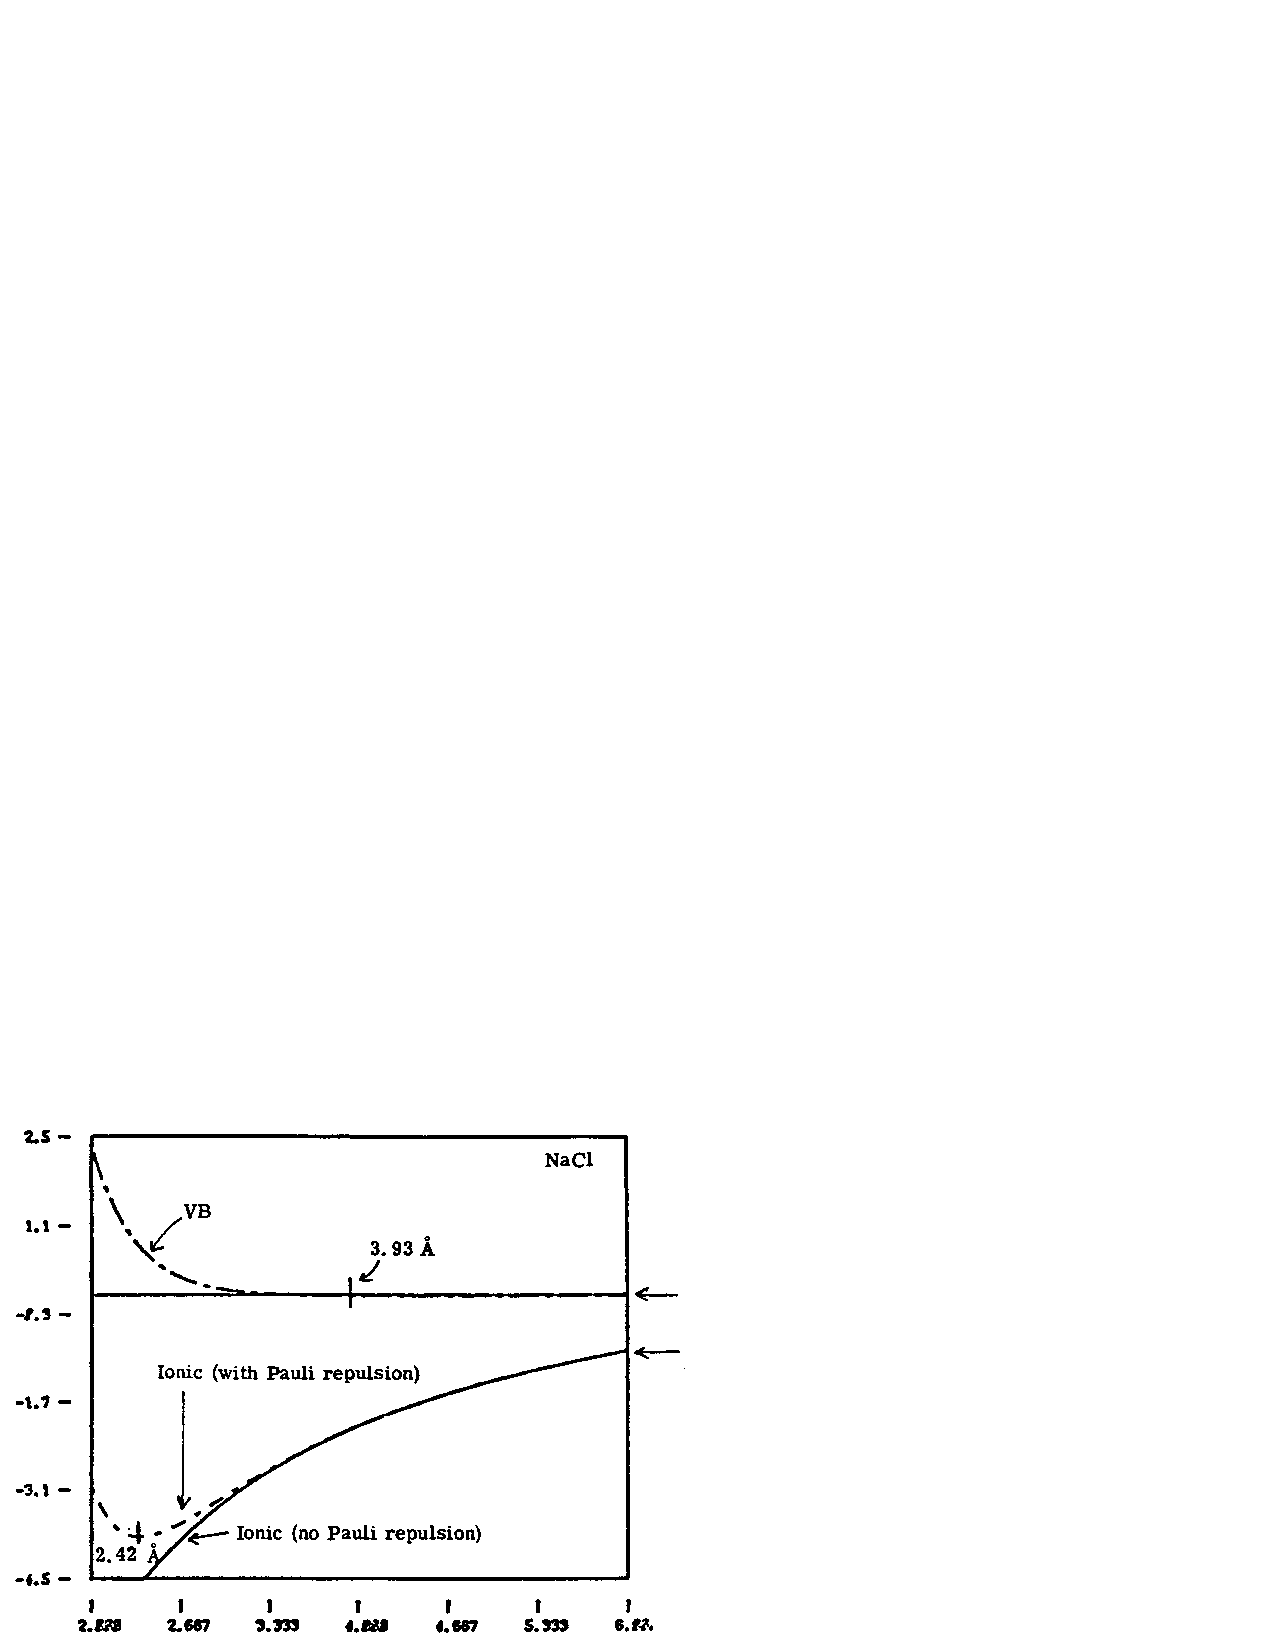
\includegraphics[scale=0.75]{fg9-01}
\caption{}
\label{chap9-fig1}
\end{figure}

Because of the low overlap and very low contragradience between
these orbitals, the bonding interactions are not able to compensate for the 
repulsive interactions arising from overlapping of nonbonding 
orbitals, e.g., Na $3s$ with Cl $3s$, Na $2p$ with Cl $3p$.

On the other hand, consider the system Na$^+$Cl$^-$ in which the
electron on the Na is ionized, energy cost = IP (Na) = 5.139 eV, and
given to the Cl, energy gain = EA(Cl) = 3.615 eV. For $R = \infty$,
energy of the ionic wavefunction is
$$
E_{ionic} ( \infty ) = E_{atom} + IP(Na) - EA(Cl) = E_{atom} + 
1.524 ~ {\rm eV}.
$$
However, at finite distances the interaction of Na$^+$ and Cl$^-$ leads to a
Coulombic attraction,
$$
E_{Coulomb}({\rm eV}) = {14.40 \over R(A)},
\label{chap9-eqno1}
$$
so that
$$
E_{ionic}(R) = E_{atom} + IP(Na) - EA(Cl) - {14.40 \over R(A)}
\label{chap9-eqno2}
$$
Substituting the experimental bond distance, $R = 2.3608$ \AA, for NaCl 
leads then to
\begin{eqnarray}
E_{ionic} (R_e) &=& E_{atom} + 1.524 - 6.100\cr 
&=& E_{atom} - 4.576 ~ {\rm eV}
\label{chap9-eqno3}
\end{eqnarray}
Indeed, the experimental bond energy is 4.23 eV, in close agreement
with this estimate.  Of course, (\ref{chap9-eqno2}) cannot be correct
for describing the energy at small $R$ since it ignores the repulsive
effects arising from the Pauli principle, ultimately leading to a
repulsive inner well in the potential. These terms depend upon the
overlap of orbitals, and have the form
$$
E_{Pauli} \approx Ae^{-BR},
\label{chap9-eqno4}
$$
where for NaCl, $A = 5920$ eV, and $B = 3.82$ \AA$^{-1}$, 
leading to an energy curve of the form
$$
E_{ionic+Pauli}(R) = E_{atom} + [IP(Na) - EA(Cl)] + E_{Pauli}(R) - 
{14.40 \over R(A)}
\label{chap9-eqno5}
$$
The formula, (\ref{chap9-eqno5}) leads to
$$
D^{calc}_0 = 3.95 ~ {\rm eV}
$$
and
$$
R_e^{calc} = 2.42 ~ {\rm \AA}
$$
as indicated in Figure \ref{chap9-fig1}, in good agreement with the
experimental values
$$
D_0^{exper} = 4.23 ~ {\rm eV} ,
$$
and
$$
R^{exper}_e = 2.361 ~ {\rm \AA}.
$$

\subsection{More Exact Descriptions}

The ground state of NaCl cannot remain ionic as the bond is pulled
apart.  The lowest energy at $R = \infty$ involves the neutrals Na and
Cl.  The way that this occurs is shown in Figure \ref{chap9-fig2},
where the optimum orbitals are shown for each $R$.  At large
distances, $R = 6$ \AA, one electron is in an Na $3s$ orbital and the
other in a Cl $3p_z$ orbital.  As $R$ decreases from $\infty$ to 4.7
\AA, the Na electron is partially shared between the Na and Cl. For
shorter distances, the electron starting on the Na becomes localized
in a $3p_z$-like orbital in the Cl.  However, for these distances, the
two electrons in the Cl $pz$ orbital are close enough to the Na$^+$ so
as to be stabilized.

\begin{figure}
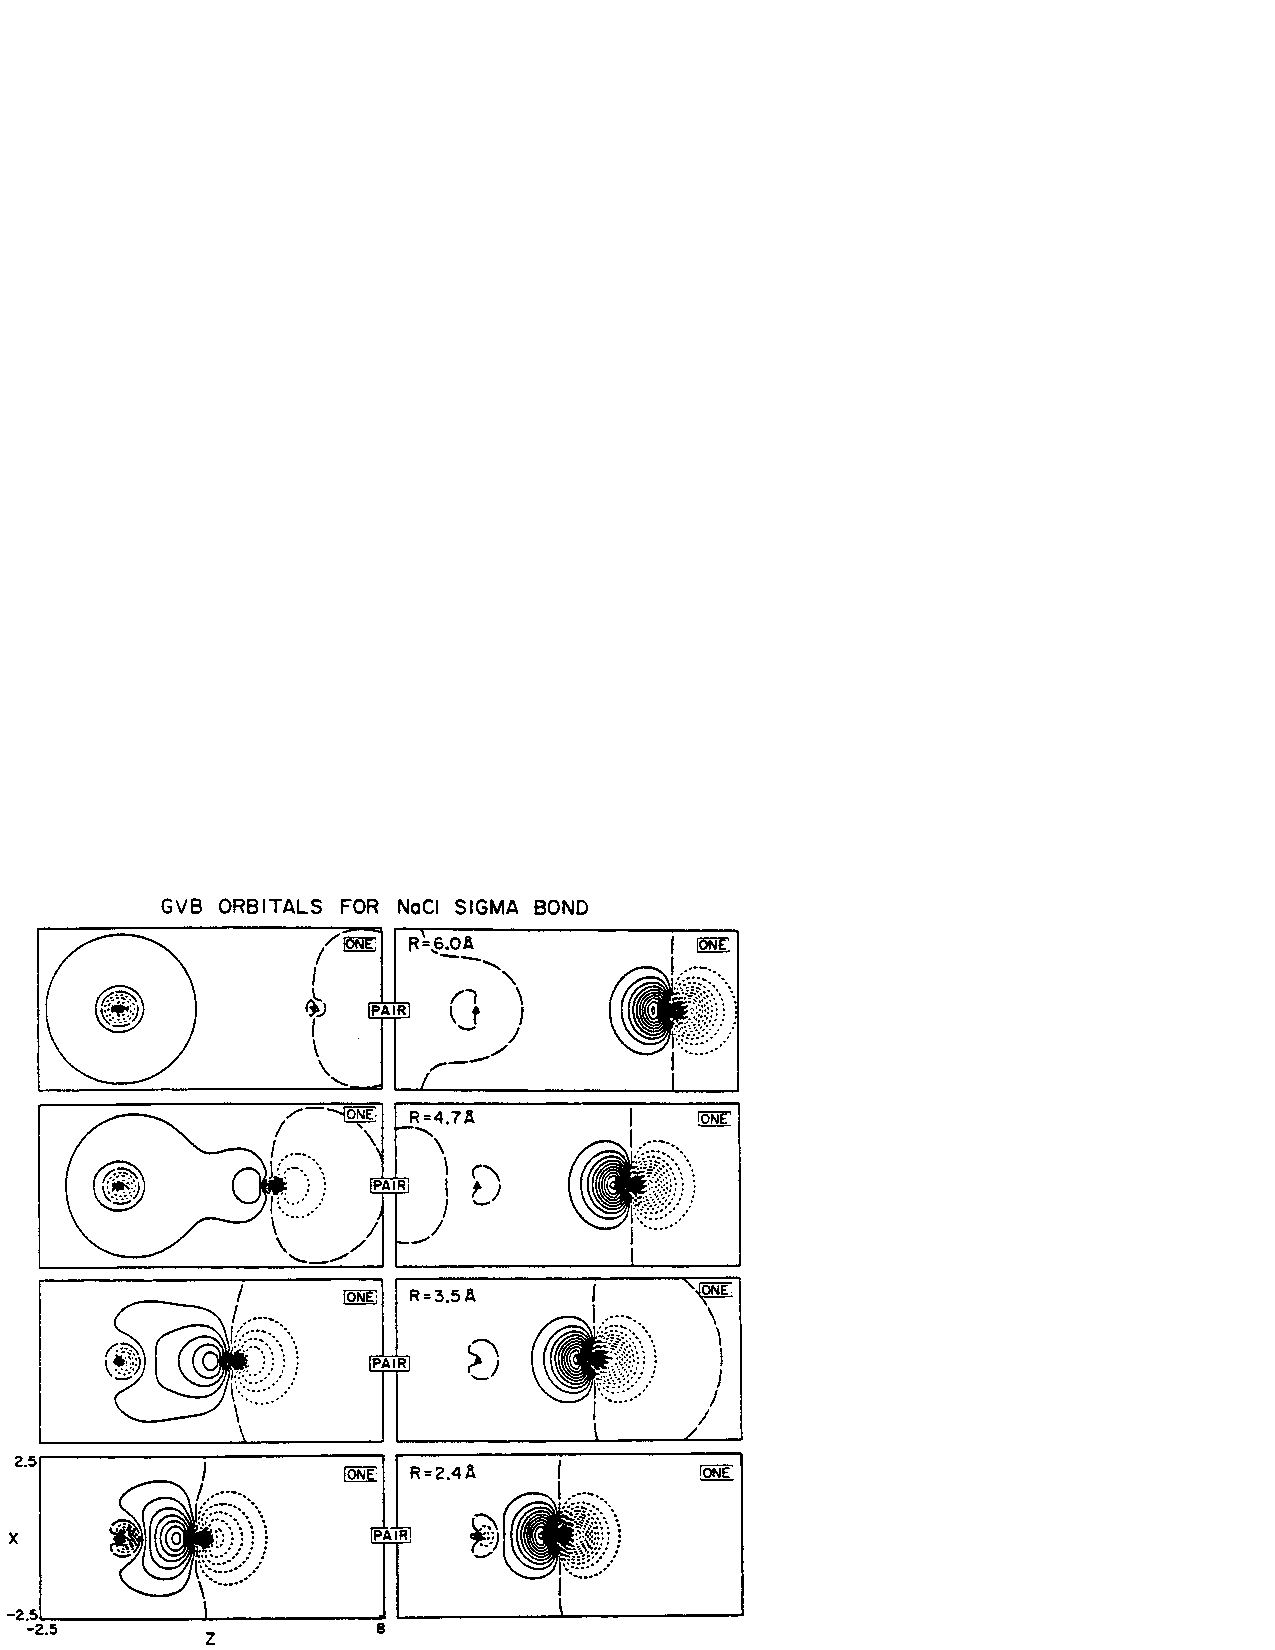
\includegraphics[scale=0.75]{fg9-02}
\caption{GVB orbitals for the NaCl $\sigma$ bond.}
\label{chap9-fig2}
\end{figure}

\subsection{Charge Transfer}

If NaCl really had the purely ionic form Na$^+$ Cl$^-$,
the dipole moment for $R = R_e$ would be $\mu = eR_e$.  In atomic 
units, this is
$$
\mu = {2.361 \over 0.529} = 4.46 ~ {\rm a.u.},
$$
and in centimeter-gram-second (cgs) units, it is
$$
\mu = (4.80310^{-10} {\rm esu}) 2.361 ~ {\rm \AA} = 11.3410^{-10} 
{\rm esu} ~ {\rm \AA} = 11.34 ~ {\rm Debye},
$$
where one 
$$
{\rm Debye} \equiv 10^{-10} ~ {\rm esu ~ \AA} = {1 \over 2.5418} ~ {\rm 
a.u.}
$$
In fact, the observed dipole moment is
$$
\mu^{obs}(NaCl) = 9.001 ~ {\rm Debye}.
$$
Thus, based on the dipole moment, we could say that 0.79 electrons transfer 
from Na to Cl in forming NaCl.  This is a clear experimental indication 
that the simple ionic description, although useful, is oversimplified.

\subsection{Interactions at Larger Distances}

\begin{figure}
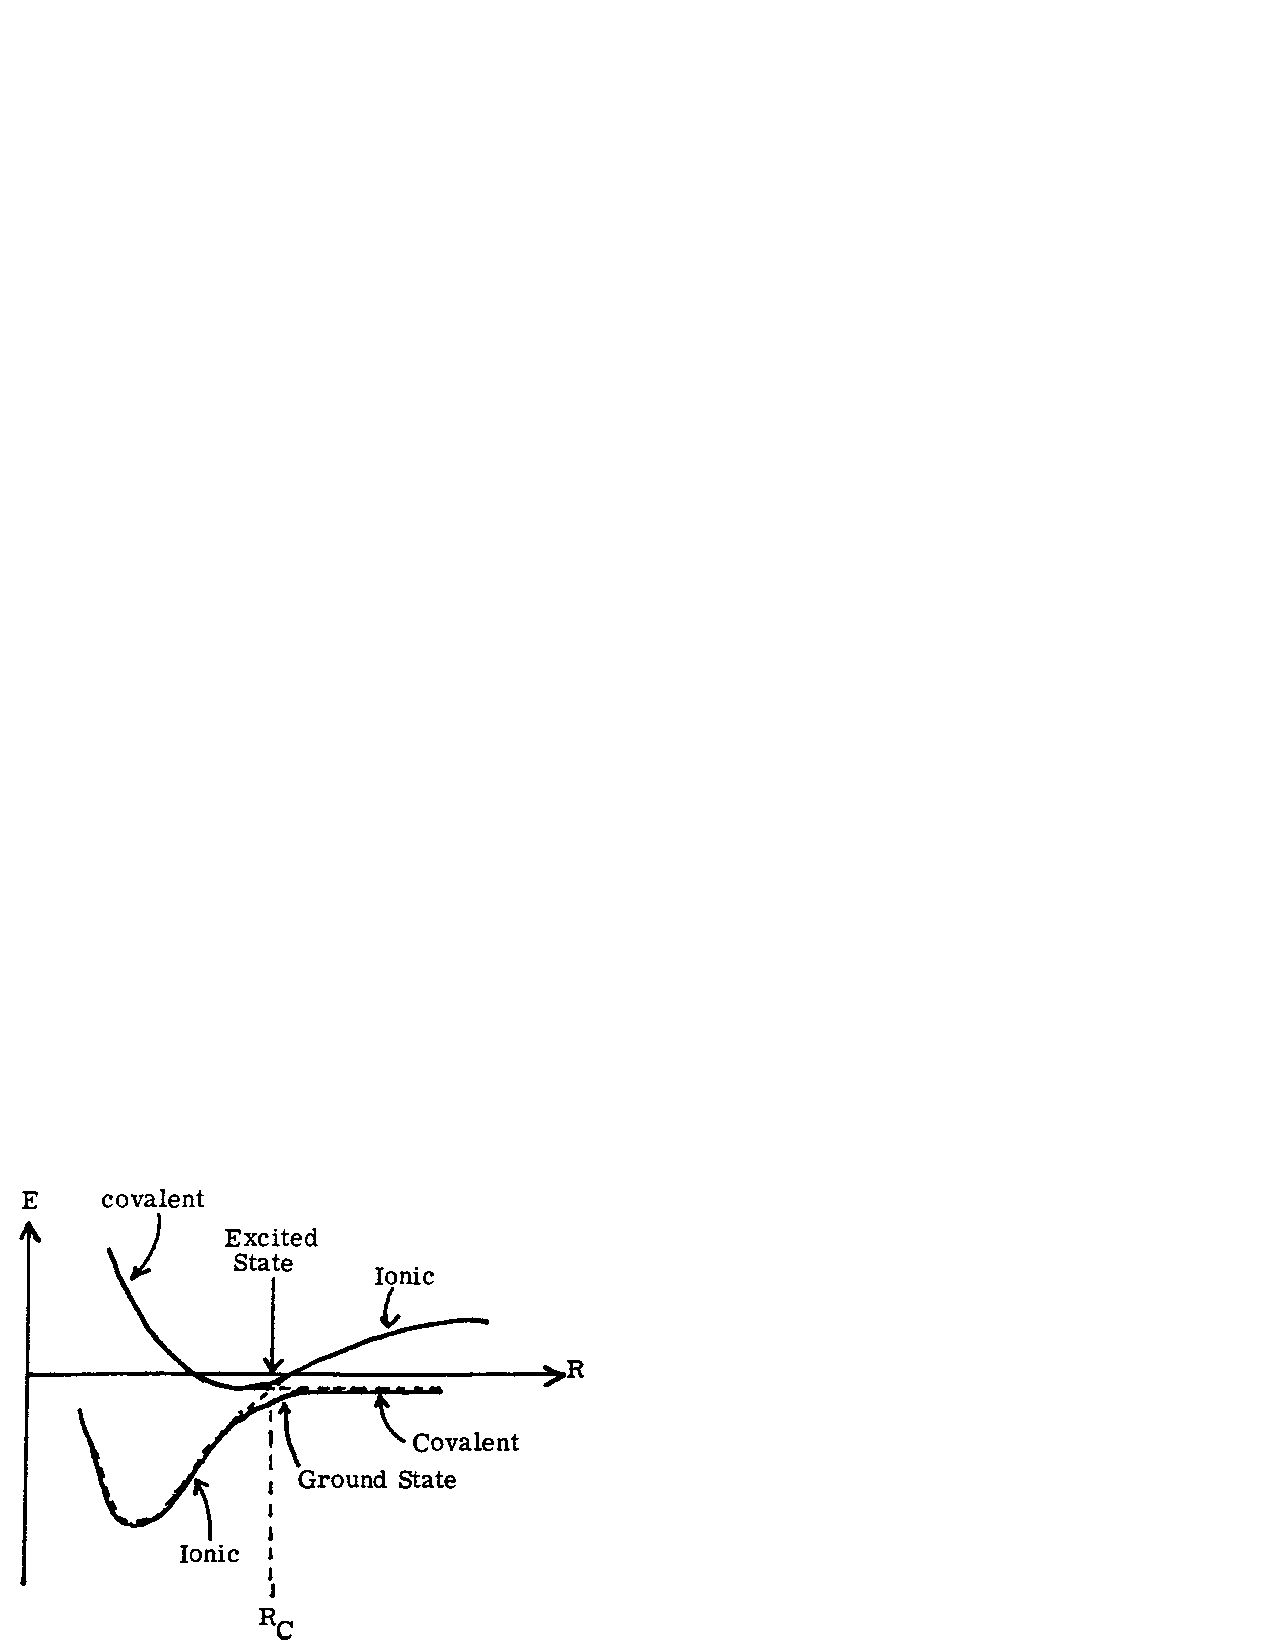
\includegraphics[scale=0.75]{fg9-03}
\caption{}
\label{chap9-fig3}
\end{figure}

Continuing the curve in Figure \ref{chap9-fig1} out to large $R$ leads
to the curve in Figure \ref{chap9-fig3}.  The ionic and covalent
wavefunctions cross at a large distance $R_e$.  This crossing point
can be calculated by assuming that the covalent curve is constant,
leading to
$$
E_{cov} = E_{Na} + E_{Cl} = E_{ion} = \left( e_{Na} + E_{Cl} + 1.524 
\right) - {14.4 \over R} ,
$$
and, hence,
$$
R_e = {14.4 \over 1.524} = 9.45 {\rm \AA} .
$$
Near this crossing point there is a strong mixing of the ionic and
covalent wavefunctions, so that the ground state changes continuously
from covalent to ionic as $R$ decreases through $R_e$.  By taking the
other, orthogonal, combination of these two wavefunctions, we obtain a
second excited state that is ionic at large $R$, and covalent at small
$R$, as indicated in Figure \ref{chap9-fig3}.

\begin{figure}
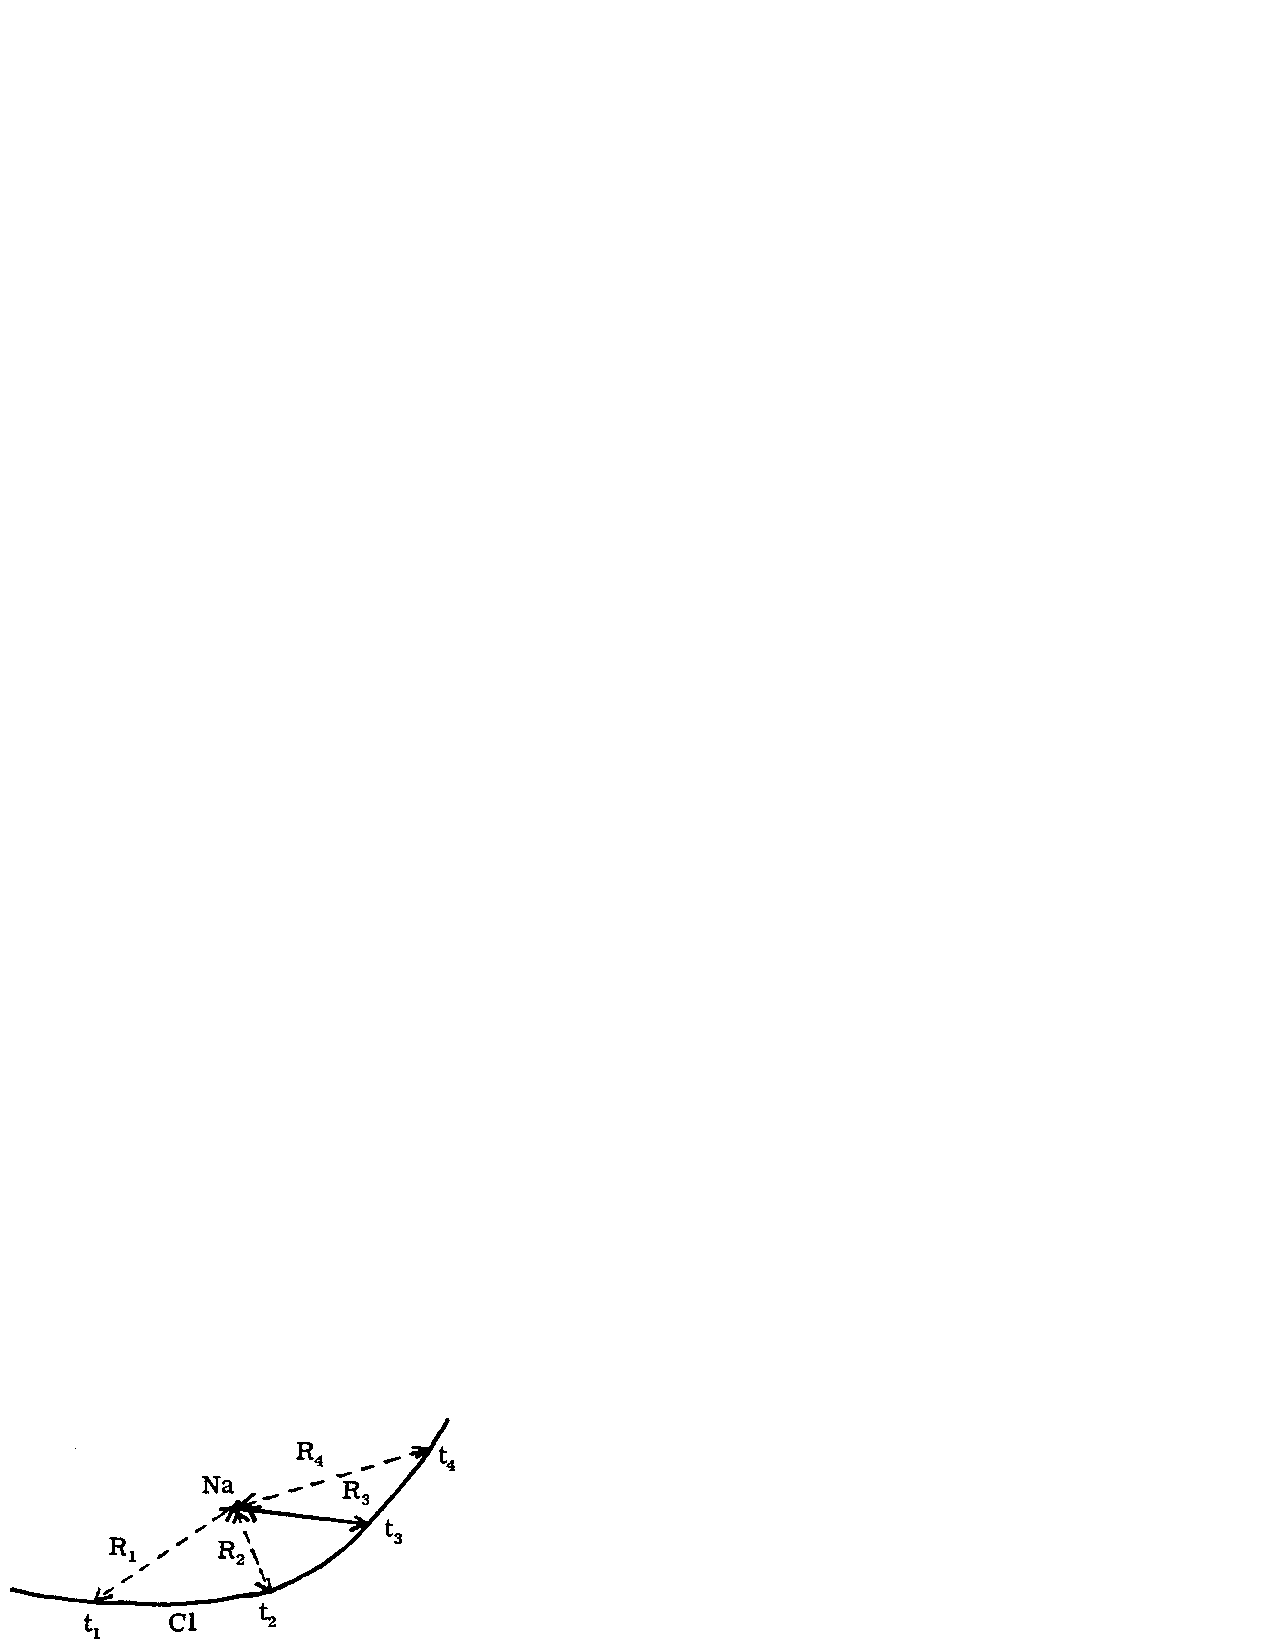
\includegraphics[scale=0.75]{fg9-04a}
\caption{}
\label{chap9-fig4a}
\end{figure}

Imagine now, a Cl atom is shot past an Na atom, as in Figure
\ref{chap9-fig4a}.  At each instant $t_i$, we can determine the force
on these atoms by using the distance $R_i$ at that instant, and
calculating
$$
F = \left[ {\partial E \over \partial R} \right]_{R_i}
$$
from Figure \ref{chap9-fig3}.  In this way, we could calculate the
path indicated in Figure \ref{chap9-fig4a}.  In terms of Figure
\ref{chap9-fig3}, the Cl would start at $R = \infty$ and would come to
some minimum $R$, $R_{min}$ in Figure \ref{chap9-fig4a}, and then go
back to $R =
\infty$, assuming no inelastic process has caused some energy to get
lost. This is indicated in Figure \ref{chap9-fig4b}. In this
description the wavefunction changes rapidly as the atom passes
through $R = R_c$ since the electron must move from the Na to the Cl.
However, if the atoms are moving sufficiently rapidly, there will not
be time for the electron to change centers, and we will find that the
forces follow the dashed, repuslive, covalent curve.  Normal
calculations of electronic wavefunctions lead to the solid curves in
Figure \ref{chap9-fig3}.  These are called \emph{adiabatic}, or
\emph{Born-Oppenheimer} potential curves, since all effects of nuclear
kinetic energy are ignored.  Including nuclear kinetic energy effects,
there is a term proportional to nuclear velocity that tends to prevent
the electronic wavefunction from changing rapidly.  This leads to the
system following the dashed curve in Figure \ref{chap9-fig3}, a
process referred to as \emph{Born-Oppenheimer breakdown}.


\begin{figure}
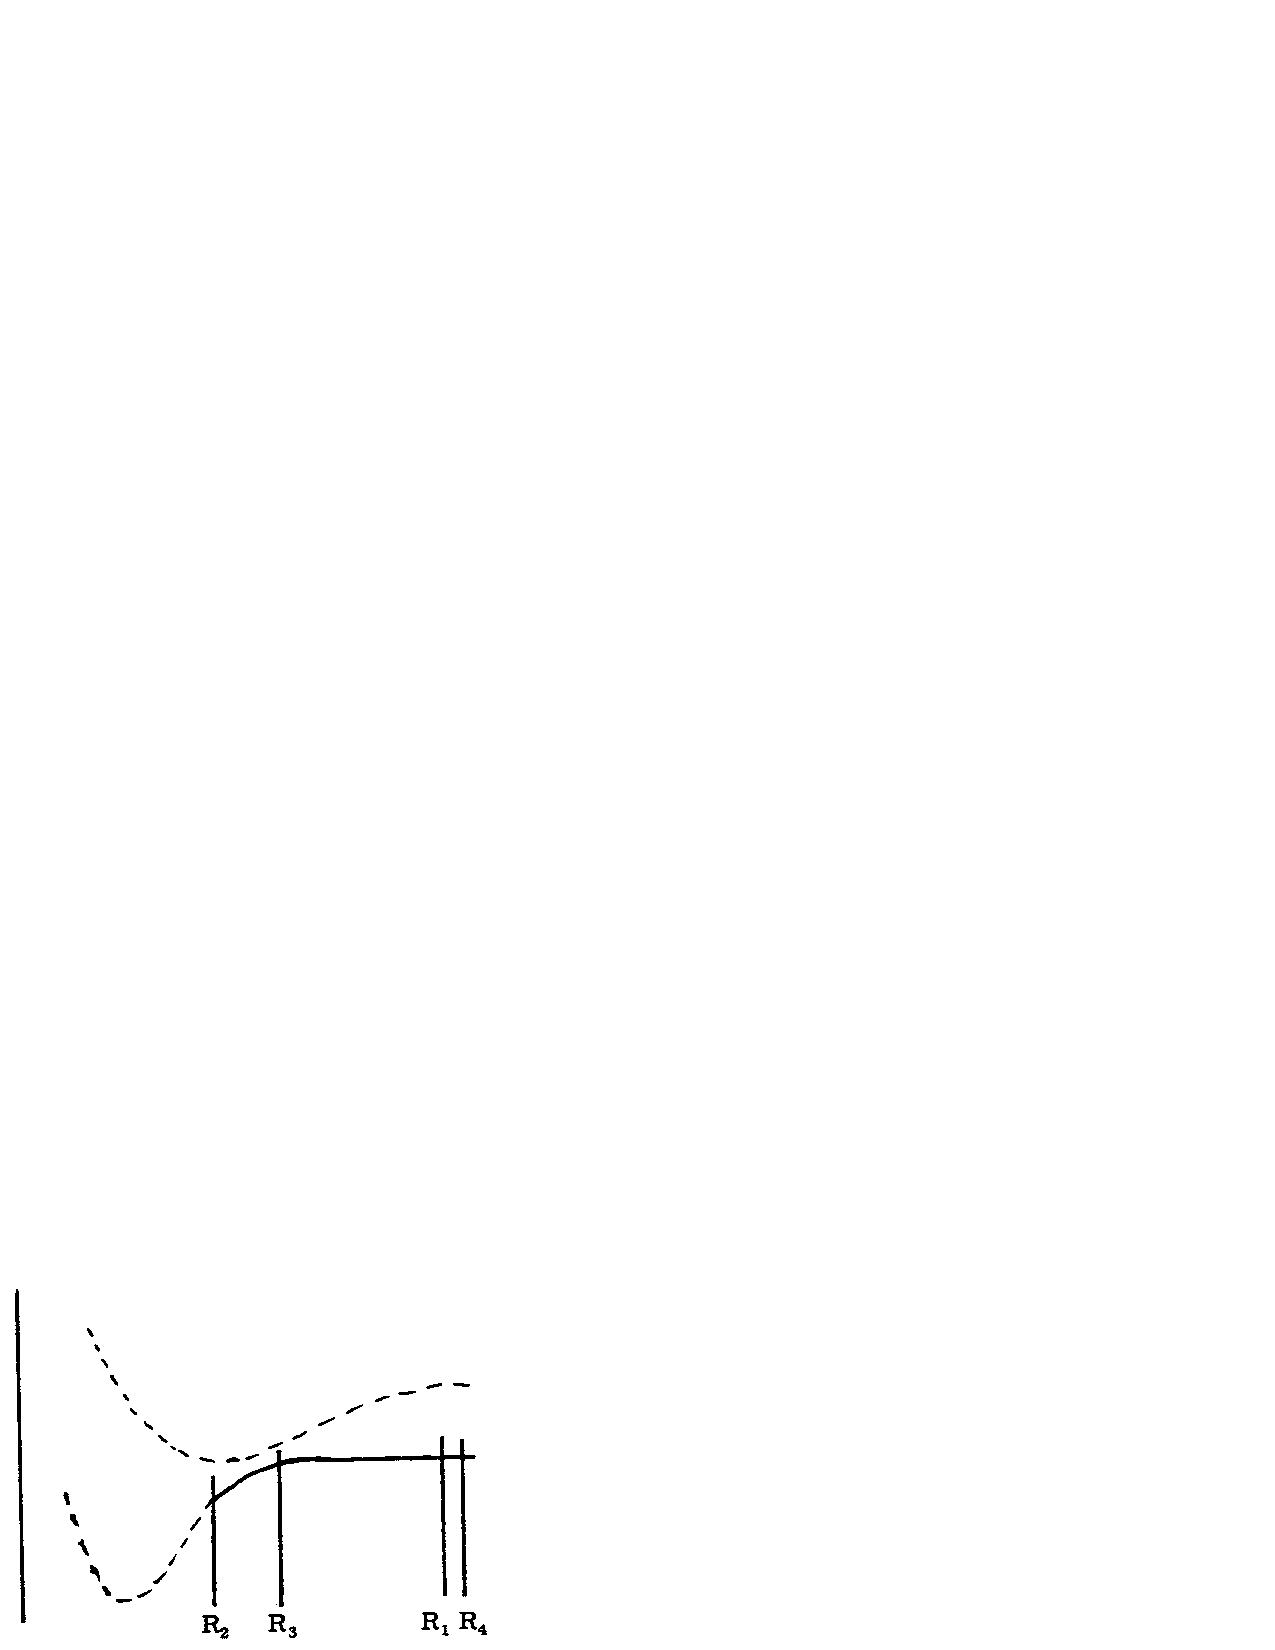
\includegraphics[scale=0.75]{fg9-04b}
\caption{}
\label{chap9-fig4b}
\end{figure}

At intermediate velocities, the electron will have time to jump from
Na to Cl as the atom approaches but not enough time to jump back as it
departs. As a result, collisions of Na and Cl may lead to products of
Na$^+$ and Cl$^-$, the energy must be above 1.5 eV for these ions to
be able to separate.  Since the crossing is at very large $R$, 9.5
\AA, the atoms need not get very close for this electron jump to
occur.  Often this process is referred to as \emph{harpooning} (the Cl
harpoons the electron from the Na) in order to emphasize the long
distances involved in the transfer.

\section{Electronegativity}

\begin{table}
\caption{Estimates of bond energies assuming purely ionic 
bonds, equation (\ref{chap9-eqno2}).  Experimental data from Herzberg
and Huber, 1980.}
\label{chap9-tab1}
\begin{tabular}{ccccccc}\\ \hline

&\multicolumn{2}{c}{Experimental}&Predicted & Error 
&\multicolumn{2}{c}{Group Average}\cr

& $R_e$ & $D_0$ & $D_{ion}$ & $D_{ion} - D_0$\cr
& (\AA) & (eV) & (eV) & (eV)\cr

LiF & 1.5639 & 5.91 & 7.22 & 1.30 & 0.68 & 0.33\cr
Na & 1.9259 & (5.3$^{\underline{3}}$) & 5.74 & 0.41 & '' & '' \cr
K & 2.1715 & 5.07 & 5.69 & 0.62 & '' & ''\cr
Rb & 2.2703 & 5.0$^{\underline{0}}$ & 5.56 & 0.56 & '' & ''\cr
Cs & 2.3454	 & 5.1$^{\underline{5}}$ & 5.64 & 0.49 & '' & ''\cr
LiCl & 2.0207 & 4.8$^{\underline{4}}$ & 5.35 & 0.51 & 0.31 & ''\cr
Na & 2.3608 & 4.23 & 4.58 & 0.35 & '' & ''\cr
K & 2.6667 & 4.34 & 4.67 & 0.33 & '' & ''\cr
Rb & 2.7867 & 4.3$^{\underline{4}}$ & 4.61 & 0.27 & '' & ''\cr
Cs & 2.9063 & 4.58 & 4.68 & 0.10 & '' & ''\cr		
LiBr & 2.1704 & 4.3$^{\underline{3}}$ & 4.6 & 0.28 & 0.19 & ''\cr
Na & 2.5020 & 3.74 & 3.98 & 0.24 & '' & ''\cr
K & 2.8208 & 3.91 & 4.13 & 0.22 & '' & ''\cr
Rb & 2.9447 & 3.9$^{\underline{0}}$ & 4.08 & 0.18 & '' & ''\cr
Cs & 3.072 & 4.17 & 4.16 & $-$0.01 & '' & ''\cr
LiI & 2.3919 & 3.51 & 3.69 & 0.15 & 0.14 & ''\cr
Na & 2.7115	& 3.00 & 3.23 & 0.23 & '' & ''\cr
K & 3.0478 & 3.31 & 3.44 & 0.13 & '' & ''\cr
Rb & 3.1769	& 3.3$^{\underline{0}}$ & 3.42 & 0.12 & '' & ''\cr
Cs & 3.3152 & 3.56 & 3.51 & $-$0.05 & '' & ''\cr
CuF & 1.7449 & 4.4$^{\underline{2}}$ & 3.93 & $-$0.49 & $-$0.52 & 
$-$1.08\cr
Ag & 1.9832 & 3.6$^{\underline{4}}$ & 3.08 & $-$0.56 & '' & ''\cr
CuCl & 2.0512 & 3.9$^{\underline{3}}$ & 2.91 & $-$1.02 & $-$0.95 & ''\cr
Ag & 2.2808 & 3.22 & 2.35 & $-$0.87 & '' & ''\cr
CuBr & 2.1734 & 3.4$^{\underline{3}}$ & 2.26 & $-$1.17 & $-$1.23 & 
''\cr
Ag & 2.3931	& 3.2 & 1.81 & $-$1.29 & '' & ''\cr
CuI & 2.3383 & $\leq$3.27 & 1.49 & $-$1.78 & $-$1.62 & ''\cr
Ag & 2.5446 & 2.6 & 1.14 & $-$1.46 & '' & ''\cr
\end{tabular}
\end{table}

For the alkali halide diatomics, the assumption of purely ionic
bonding leads to fairly accurate predictions of bond energies, as
indicated in Table \ref{chap9-tab1}. Of course, these predictions make
use of the experimental $R_e$.  For the copper halides and the silver
halides, such predictions lead to bond energies too small, since we
are ignoring the Pauli terms, the ionic description, if correct, would
lead to too large a bond energy, and for most other molecules the
ionic model leads to very inaccurate predictions.  One problem here is
that even in the alkali halides there is certainly some sharing of
electrons, see Figure \ref{chap9-fig2}.  Thus, the observed dipole moments
correspond to a charge transfer of only about 0.8 electrons.
Compounding this problem, different atoms have different affinities
for electrons so that the amount of charge transfer should be
different for each pair of electrons.  To illustrate this, some
properties of various diatomics formed from alkalis, halogens, and
hydrogen are listed in Table \ref{chap9-tab2}. In Table
\ref{chap9-tab3} we list the fractional ionic character of various
bonds based on the observed dipole moments.

\begin{table}
\caption{Properties of heteronuclear diatomic molecules.}
\label{chap9-tab2}
\begin{tabular}{ccccc}\\ \hline

& $R_e$$^a$ & $\omega_e$$^b$ & $\mu_o$$^a$ & $D_o$$^c$\cr
& (\AA) & (cm$^{-1}$) & (D) & (eV)\cr

BrC & 2.136 & & 0.57 & 2.23??\cr
BrCs & 3.072 & & 10.82 & 4.07?\cr
BrF & 1.756 & & 1.29 & 2.384\cr
BrH & 2.415 & & 0.828 & 3.75?\cr
BrI & 2.485 & & -- & 2.817\cr
BrK & 2.821 & & 10.626 & 3.94?\cr
BrLi & 2.022 & & 7.268 & 4.35?\cr
BrNa & 2.502 & & 9.118 & 3.8?\cr
BrRb & 2.945 & & 10.86 & 4.0?\cr
C$\ell$Cs & 2.906 & & 10.387 & 4.55?\cr
C$\ell$F & 1.628 & & 0.888 & 2.558\cr
C$\ell$H & 1.275 & & 1.109 & 4.431\cr
C$\ell$I & 2.321 & & 1.24 & 2.152\cr
C$\ell$K & 2.667 & & 10.269 & 4.36?\cr
C$\ell$Li & 2.021 & & 7.129 & 4.9??\cr
C$\ell$Na & 2.361 & & 9.001 & 4.25?\cr
C$\ell$Rb & 2.787 & & 10.510 & 4.4??\cr
CsF & 2.345 & & 7.884 & 5.33?\cr
CsH & 2.494$^b$ & 891.29 & -- & 1.8??\cr
CsI & 3.315 & & 11.69 & 3.4??\cr
FH & 0.917 & & 1.827 & 5.84?\cr
FI & 1.910 & & -- & 2.87?\cr
FK & 2.171 & & 8.593 & 5.07?\cr
FLi & 1.564 & & 6.327 & 5.95?\cr
FNa & 1.926 & & 8.156 & 4.95?\cr
FRb & 2.270 & & 8.547 & 5.2??\cr
HI & 1.609 & & 0.448 & 3.06?\cr
HK & 2.242$^b$ & 983.63 & -- & 1.86?\cr
HLi & 1.595 & & 5.884 & 2.429\cr
HNa & 1.887$^b$ & 1172.2 & -- & 2.05?\cr
HRb & 2.367$^b$ & 936.94 & -- & 1.7??\cr
IK & 3.048 & & 10.82 & 3.4??\cr
ILi & 2.392 & & 7.429 & 3.57?\cr
INa & 2.711 & & 9.236 & 3.05?\cr
IRb & 3.177 & & 11.48 & 3.47?\cr
NaK & -- & 123.29 & -- & 0.62?\cr
NaRb & -- & 106.64 & -- & 0.57?\cr
\hline
\end{tabular}\\
$^a$ Unless indicated otherwise, all values are from	J. Phys.
Chem. Res. Data, 1974.
$^b$ From Rosen.
$^c$ From Gaydon,
\end{table}

In order to provide a measure for predicting how polar various bonds should 
be, Linus Pauling$^1$ developed a scale of electronegativities where the 
atom that gains extra charge is said to be more electronegative and the 
one that loses charge is said to be more electropositive.  The greater the 
difference in electronegativity, the greater the ionic character in
the bond.

One measure used, for the ionic character in the bond, is the dipole 
moment, vide supra.  Pauling$^1$ suggested the relationship
$$
{\rm amount ~ ionic ~ character} = 1 - e^{-[(\chi_A - 
\chi_B)/4]}
\label{chap9-eqno6}
$$
which provides very rough agreement with experiment.  A second criterion 
involved ionic contributions to bond energies, vide infra. The final 
electronegativities are given in Table \ref{chap9-tab4}.

\begin{table}
\caption{Fractional ionic character of bonds, obtained 
from $\Delta q = \mu$(a.u.)/$R$(a.u.) = $C \mu(D)/R$(\AA) where $C$ =
0.743470. Positive implies that the head of the column is more
electronegative.}
\label{chap9-tab3}
\begin{tabular}{cccccc}\\ \hline

& F & Cl & Br & I & H\cr

F & 0.0 & $-$0.1136 & $-$0.1529 & -- & $-$0.4148\cr
Cl & 0.1136 & 0.0 & $-$0.0556 & $-$0.1112 & $-$0.1811\cr
Br & 0.1529 & 0.0556 & 0.0 & -- & $-$0.1218\cr
I & -- & 0.1112 & -- & 0.0 & $-$0.0579\cr
H & 0.4148 & 0.1811 & 0.1218 & 0.0579 & 0.0\cr
Li & 0.8423 & 0.7345 & 0.7485 & 0.6466 & 0.7678\cr
Na & 0.8816 & 0.7938 & 0.7587 & 0.7092\cr
K & 0.8238 & 0.8017 & 0.7844 & 0.7391\cr
Rb & 0.7837 & 0.7852 & 0.7678 & 0.7523\cr
Cs & 0.6998 & 0.7441 & 0.7333 & 0.7341\cr
\hline
\end{tabular}
\end{table}

\begin{table}
\caption{Comparison of Mulliken, and Pauling electronegativities,
alkali and halogen atoms.}
\label{chap9-tab5}
\begin{tabular}{ccccc}\\ \hline

& IP$^a$ & EA$^b$ & X$_{Mulliken}$$^c$ & X$_{Pauling}$\cr
& (eV) & (eV)\cr

F & 17.422 & 3.399 & 4.00 & 4.0\cr
Cl & 12.967 & 3.615 & 3.19 & 3.0\cr
Br & 11.814 & 3.364 & 2.92 & 2.8\cr
I & 10.451 & 3.061 & 2.60 & 2.5\cr
H & 13.598 & 0.75421 & 2.76 & 2.1\cr
Li & 5.392 & 0.620 & 1.15 & 1.0\cr
Na & 5.239 & 0.546 & 1.09 & 0.9\cr
K & 4.341 & 0.501 & 0.93 & 0.8\cr
Rb & 4.177& $\sim$0.486 & 0.90 & 0.8\cr
Cs & 3.894 & $\sim$0.472 & 0.84 & 0.7\cr
\hline
\end{tabular} \\
$^a$ From NSRDS-NBS 34. 
$^b$ H. Notep and W. C. Lineburger, J. Phys. Chem. Ref. 
Data, Volume 4, page 539, 1975.
$^c$ (IP + EA)/5.2053.
\end{table}

As expected, the charge transfer, Table \ref{chap9-tab3}, increases
nearly monotonically with the electronegativity difference. Note that
nearly all alkali halides have between 70 and 90 percent ionic
character. Unfortunately, this definition of $\Delta q$ has flaws
since, for example, it does not take into account the contribution to
the dipole moment arising from hybridization of the orbitals, which
may be quite large.

Mulliken formulated another set of electronegatives based solely upon the 
properties of the atoms
$$
\chi^M = {(IP + EA) \over 5.2}
$$
where $IP$ is the ionization potential of an atom and $EA$ is the
electron affinity, positive values indicating that the atom will
accept an electron. The 5.2 is a normalization factor so that
$\chi^M(F) = 4.0$, just as on the Pauling scale.  The final values for
a selection of atoms are listed in Table \ref{chap9-tab5}, where they
are compared with the Pauling values. The Pauling and Mulliken values
compare well except for H.  Comparing with the properties of the
molecules, e.g., $\Delta q(HI)$ in Table \ref{chap9-tab4}, it seems
clear that the Pauling value for $\chi_H$ is the better choice.

Note that the most electronegative elements are in the upper right hand 
corner of the periodic table in the order F, O, with N and Cl tied for 
third, Br next, and then a tie between C, S, and I, while the most 
electropositive elements are in the lower left hand corner, Cs and Fr.

\subsection{Ionic Contributions to Bonding}

Pauling assumed for a covalent bond between atoms A and B, that the bond
energies are related by
$$
D(A - B) = \sqrt{D(A-A) \cdot D(B-B)}.
\label{chap9-eqno7}
$$
This can be derived by assuming that bond energies are proportional to 
orbital overlaps.  The long-range form for an atomic $n \ell$ orbital 
is $\varphi_{n \ell} \approx e^{- \zeta r}$, where $\zeta = 1/n 
\sqrt{2IP}$, and the $IP$ is in atomic units.  Consequently, the 
overlap of the orbital on two atoms, $a$ and $b$, behaves approximately as
$$
S_{ab}  = e^{-\sqrt{\zeta_a \zeta_b R}}.
$$
If the bond energy $D_{ab}$ is proportional to $S_{ab}$, $D_{ab} = 
\eta S_{ab}$, we then obtain
$$
{D_{ab} \over \sqrt{D_{aa} D_{bb}}} = {S_{ab} \over \sqrt{S_{aa} 
S_{bb}}} = 1,
$$
leading to (\ref{chap9-eqno7}).  Writing the actual bond energy as
$$
D(A-B) = \sqrt{D(A-A) \cdot D(B-B)} + \Delta (A-B).
\label{chap9-eqno8}
$$
Pauling attributed the extra bond energy $\Delta (A-B)$ to the ionic nature 
of the bond. His tables of electronegativities were then adjusted to 
fit, approximately
$$
\Delta (A-B ) = 30 ( \chi_A - \chi_B)^2.
\label{chap9-eqno9}
$$

Table \ref{chap9-tab6} contains the ionic contributions to the bond
energy defined as
$$
\Delta(A-B) = D(A-B) - \sqrt{D(A-A) \cdot D(B-B)}.
\label{chap9-eqno10}
$$
This table is based on Tables \ref{chap9-tab2} and \ref{chap9-tab7}.
As expected, this is large for cases with large electronegativity
differences.
\begin{table}
\caption{Ionic contribution to the bond energy, m eV.  Defined 
as $\Delta(A - B) = D(A-B) - \sqrt{D(A-A) \cdot D(B-B)}$.}
\label{chap9-tab6}
\begin{tabular}{cccccc}\\ \hline

& F & Cl & Br & I & H\cr

F & 0.0\cr
Cl & 0.538 & 0.0\cr
Br & 0.606 & 0.02 & 0.0\cr
I & 1.30 & 0.197 & 0.073 & 0.0\cr
H & 2.16 & 1.101 & 0.78 & 0.43 & 0.0\cr
Li & 4.61 & 3.2 & 2.86 & 2.25 & 0.19\cr
Na & 3.85 & 2.89 & 2.6 & 1.98 & 0.22\cr
K & 4.16 & 3.24 & 2.94 & 2.5 & 0.35\cr
Rb & 4.3 & 3.3 & 3.0 & 2.62 & 0.25\cr
Cs & 4.48 & 3.49 & 3.1 & 2.6 & 0.38\cr
\hline
\end{tabular}
\end{table}


\subsection{Ionic Contributions to Bond Distance}

\begin{table}
\caption{Properties of homonuclear diatomic molecules.}
\label{chap9-tab7}
\begin{tabular}{cccccc}\\ \hline
& $R_e$$^a$ & $\omega_e$$^a$ & $D_0$$^b$ & $D_0$ & IP$^a$\cr
& (\AA) & (cm$^{-1}$) & (eV) & (kcal) & (eV)\cr

F$_2$ & 1.417 & 891.8$_5$ & 1.60$_5$ & 37.7\cr
Cl$_2$ & 1.9878	& 559.71 & 2.476 & 57.18 & 11.48\cr
Br$_2$ & 2.2809	& 323.33 & 1.970 & 45.44 & 10.55\cr
I$_2$ & 2.667 & 214.52 & 1.5439 & & 9.28\cr
H$_2$ & 0.74116	& 4403.19 & 4.4773\cr
Li$_2$ & 2.67 & 351.35 & 1.12 & 26.3\cr
Na$_2$ & 3.08 & 159.23 & 0.75 & 17.2\cr
K$_2$ & & 3.92$_3$ & 92.64 & 0.51\cr
Rb$_2$ & & 57.31 & 0.4$_7$ & 11.3\cr
Cs$_2$ & & & 0.45 & 10.4\cr
F$^+_2$ & (1.326) & & & 73.5\cr
Cl$^+_2$ & 1.8917 & 645.61 & & 99.2\cr
H$^+_2$ & 1.06 & 2297\cr
Li$^+_2$\cr
Na$^+_2$\cr
\hline
\end{tabular}\\
$^a$ From Rosen.
$^b$ From Gaydon.
\end{table}

Experimental values for various properties of diatomic molecules are
given in Tables \ref{chap9-tab2} and \ref{chap9-tab7}.  Here, $R_e$ is
the bond length for the minimum in the potential curve; $\omega_e =
\sqrt{k_e/\mu}$ is related to the force constant $k_e$ at $R_e$, and
$\mu$ is the reduced mass; $D_0$ is the bond dissociation energy from
the $v = 0$ level, thus, this does not include the zero point energy;
IP is the ionization potential.

Using Table \ref{chap9-tab2}, we obtain the values in Table
\ref{chap9-tab8} as the bond radii for covalent bonds.  In Table
\ref{chap9-tab9}, we compare these actual bond lengths with the
predictions from Table \ref{chap9-tab8},
$$
\Delta R = R_{AB} - {1 \over 2} \left( R_{AA} + R_{BB} 
\right).
\label{chap9-eqno11}
$$
For nearly all cases, $\Delta R$ is negative so that increased ionic 
character in the bond leads to a decrease in the bond length.  The 
magnitude of $\Delta R$ increases roughly with the
electronegativity difference.

\begin{table}
\caption{Covalent bond radii.}
\label{chap9-tab8}
\begin{tabular}{cc}\\ \hline

& $R_e$ in \AA$^a$\cr

F & 0.709\cr
Cl & 0.994\cr
Br & 1.141\cr
I & 1.334\cr
H & 0.371\cr
Li & 1.33$_5$\cr
Na & 1.54\cr
K & 1.96$_2$\cr
Rb & (2.10)$^b$\cr
Cs & (2.25)$^b$\cr
\hline
\end{tabular}\\
$^a$ From Table \ref{chap9-tab7}.
$^b$ Based on comparison of RbX, CsX, and KX molecules with X = 
Cl, Br, I, and H, including the idea that K, Rb, and Cs become 
successively more electronegative.
\end{table}

\begin{table}
\caption{Comparison, in \AA, of actual bond length with 
predicted value from adding the covalent radii.  Negatives imply an
actual bond length less than the predicted value.}
\label{chap9-tab9}
\begin{tabular}{cccccc}\\ \hline

& F & Cl & Br & I & H\cr

F & 0.0\cr
Cl & $-$0.074 & 0.0\cr
Br & $-$0.093 & $-$0.146 & 0.0\cr
I & $-$0.132 & $-$0.191 & +0.011 & 0.0\cr
H & $-$0.162 & $-$0.090 & $-$0.096 & $-$0.095 & 0.0\cr
Li & $-$0.480 & $-$0.308 & $-$0.454 & $-$0.277 & $-$0.111\cr
Na & $-$0.323 & $-$0.173 & $-$0.179 & $-$0.163 & $-$0.024\cr
K & $-$0.500 & $-$0.289 & $-$0.282 & $-$0.248 & $-$0.091\cr
Rb & $-$0.54 & $-$0.31 & $-$0.30 & $-$0.26 & $-$0.10\cr
Cs & $-$0.61 & $-$0.34 & $-$0.32 & $-$0.27 & $-$0.13\cr
\hline
\end{tabular}\\
$^a$ See footnote $b$ of Table \ref{chap9-tab8}.
\end{table}

\section{Ionic Crystals}

\subsection{Monovalent Ionic Structures}

Earlier, we saw that diatomic molecules such as NaCl involve nearly 
complete charge transfer so that the molecule can be thought of as 
Na$^+$Cl$^-$.  Bonding together two such
molecules, leads to a tightly bound direct,
\begin{equation}
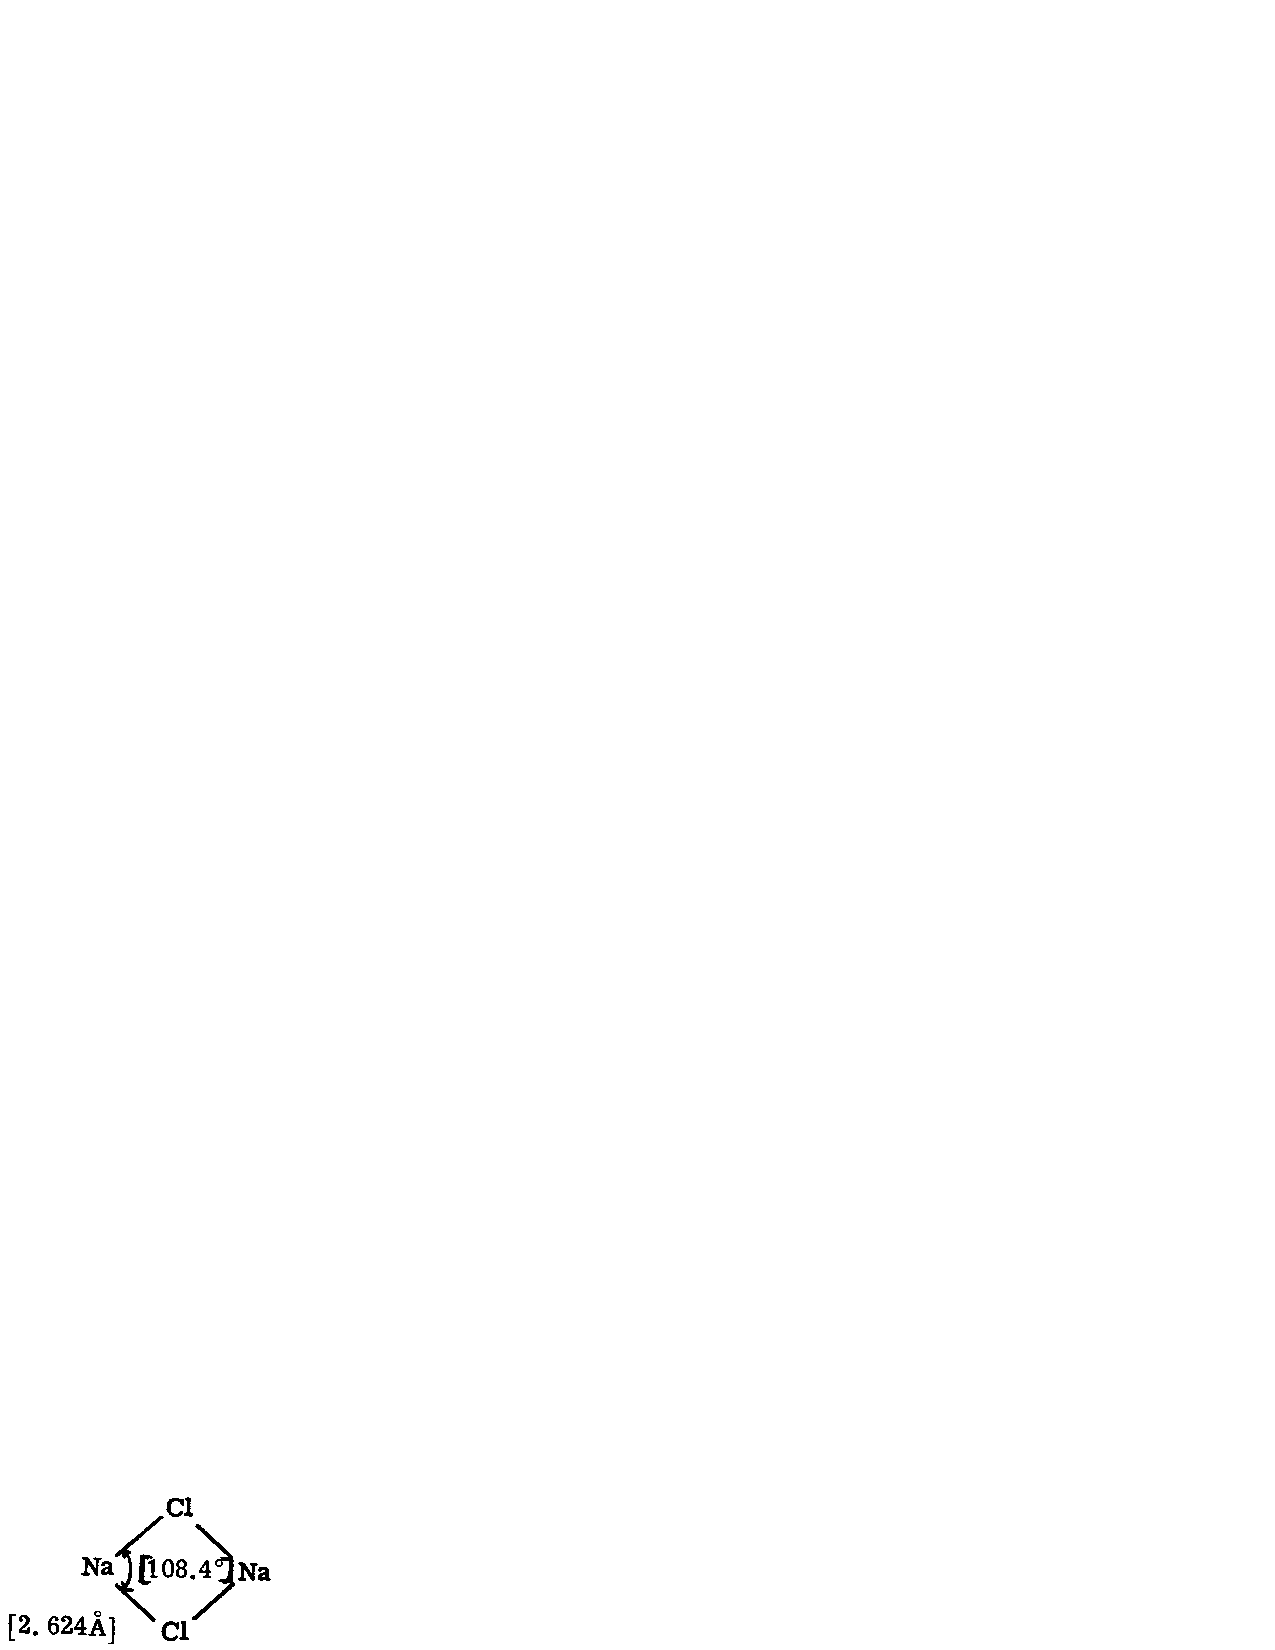
\includegraphics{fg9-04c}
\label{chap9-eqno12}
\end{equation}
in which each atom is bonded equally to two others.  Because of the presence 
of electrostatic repulsions between like charges, the bond lengths are 
0.26 \AA\ larger than in the monomer. The bond energy of the dimer, relative 
to the monomer, is 2.10 eV$^2$, at 0$^{\circ}$K), in reasonable
agreement with the purely electrostatic estimate of 1.68 eV. Dimer
$$
E_{elect} = \left[ - {4 \over 2.624} + {1 \over 3.070} + {1 \over 
4.256} \right] 14.4 = 13.88 {\rm eV}.
$$
Monomer
$$
E_{elect} = - {14.4 \over 2.361} = - 6.10 {\rm eV}.
$$

Similarly, two dimers combine to form a strongly bonded tetramer,
\begin{equation}
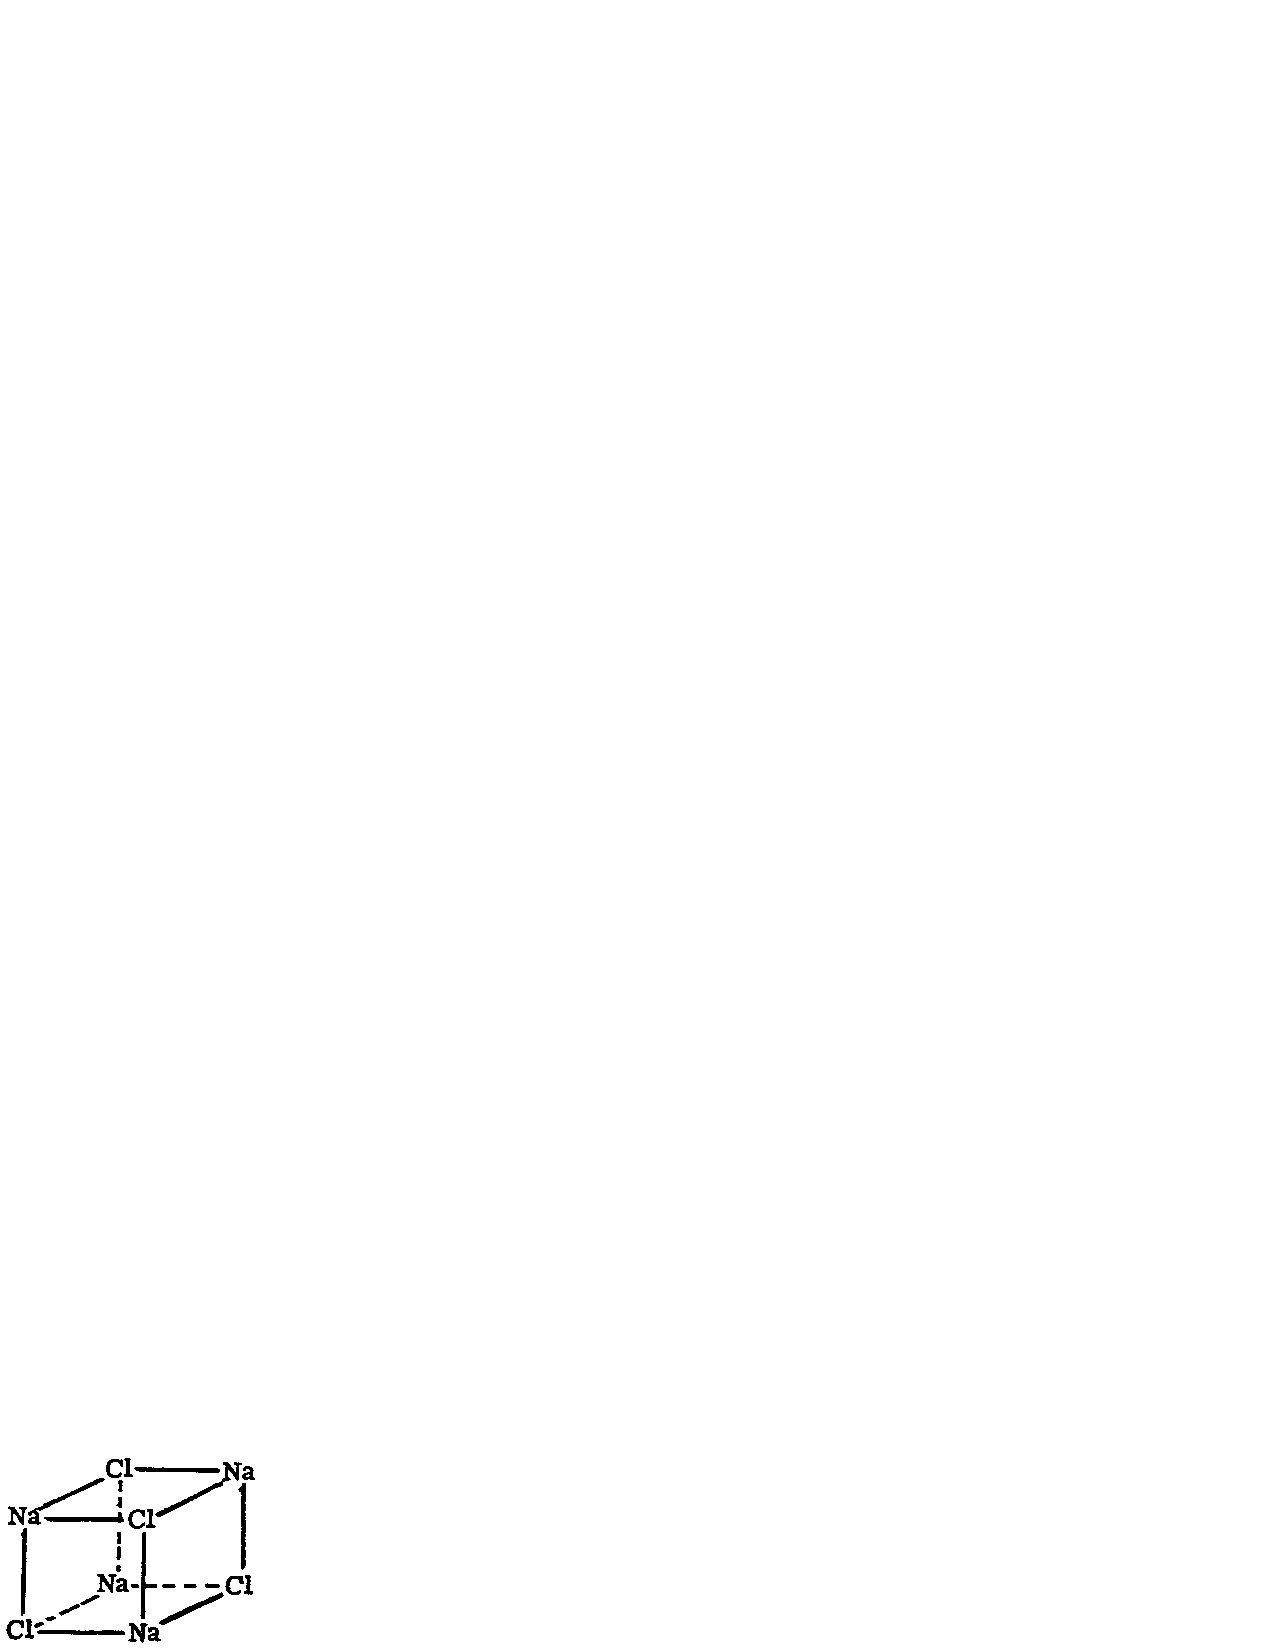
\includegraphics{fg9-04d}
\label{chap9-eqno13}
\end{equation}
and $4(10^{18})$ such dimers make a grain of salt in which the
arrangement of atoms is as given in Figure \ref{chap9-fig5}, where
each Na has six Cl neighbors and each Na has six Cl neighbors

\begin{figure}
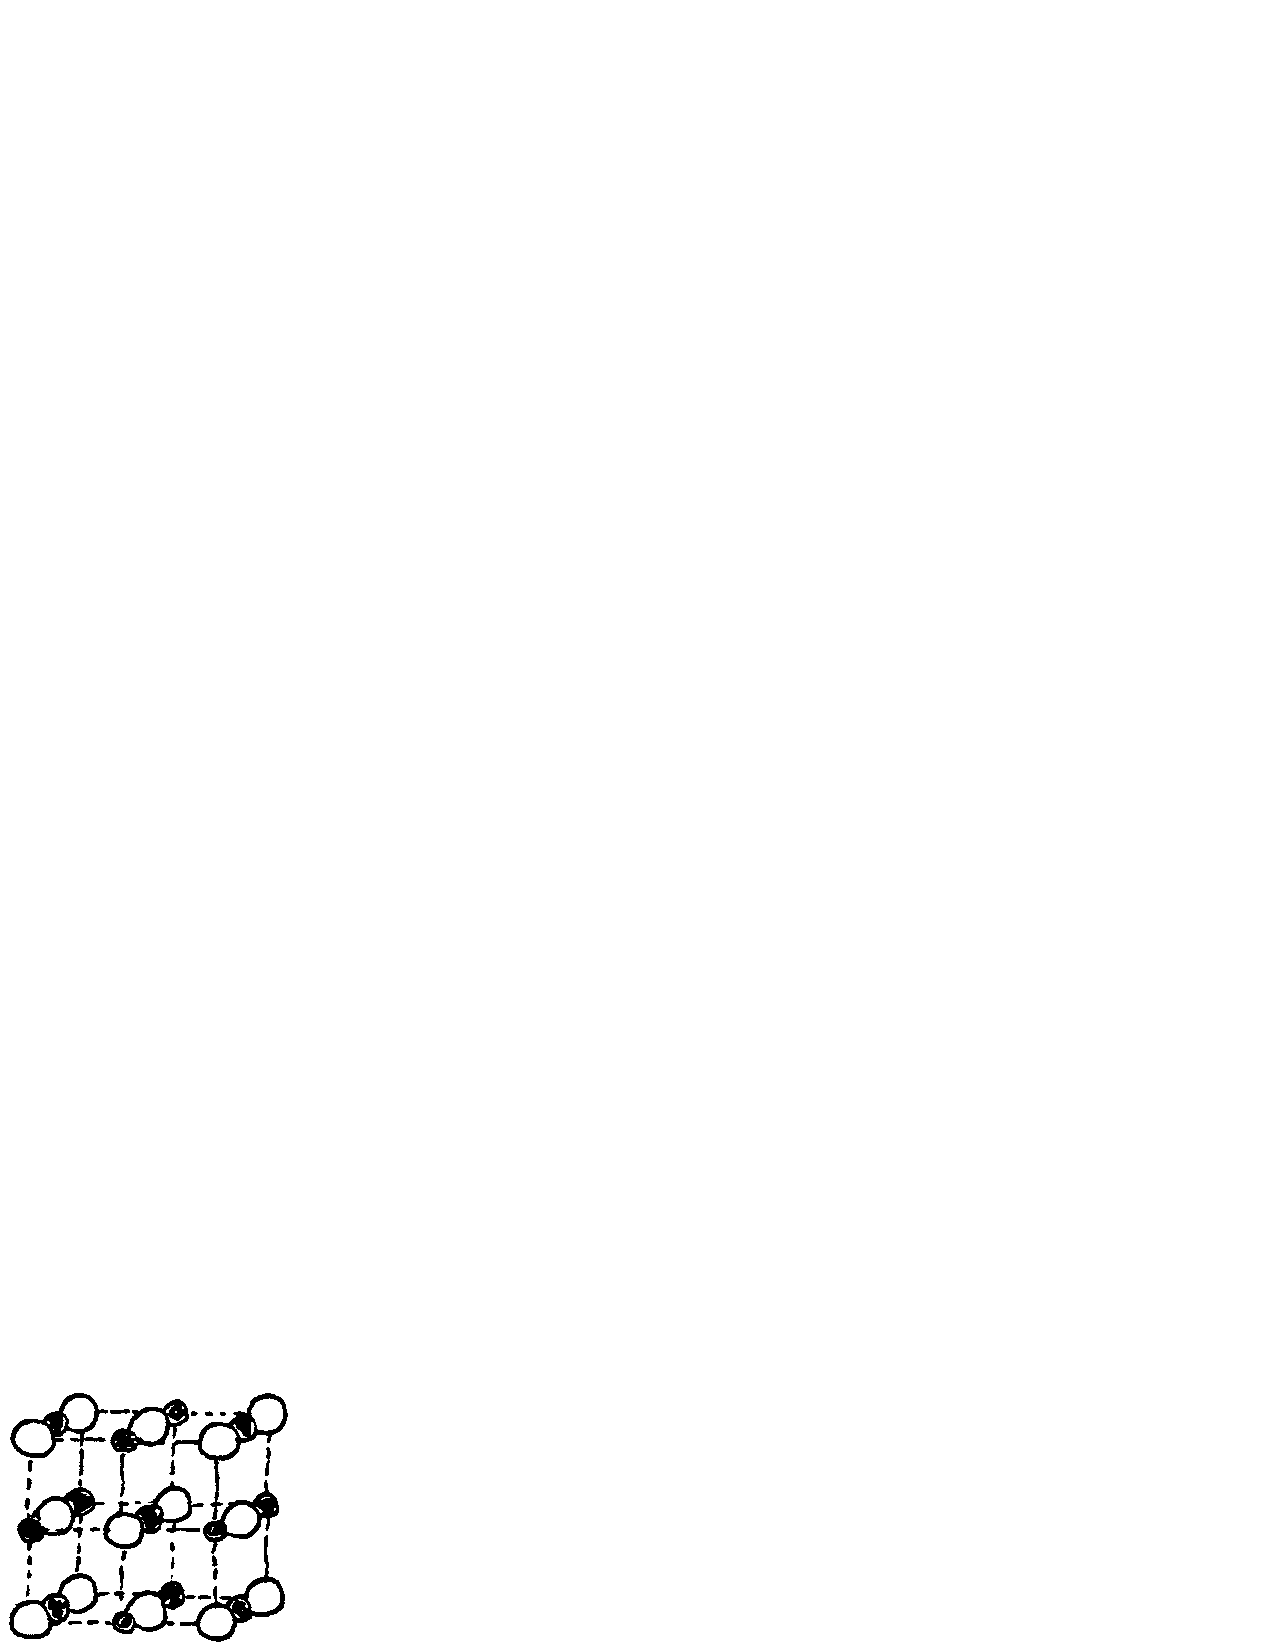
\includegraphics[scale=0.75]{fg9-05}
\caption{The NaCl structure (B1). In such systems, the bonding is best
thought of in terms of interactions of isolated cations and anions,
rather than the localized two-electron bonds characteristic of Si and
GaAs.}
\label{chap9-fig5}
\end{figure}


Starting with a cubic unit cell of length $a$, the Na
are placed at the center, $({1 \over 2}a, {1 \over 2} a, {1 \over 
2}a)$, and at the center of each edge, $(0 , 0 , {1 \over 2}a)$, 
$(0 , {1 \over 2}a , 0)$, $({1 \over 2} a , 0 , 0)$, 
the Cl are at the corners (0,0,0) and at the center of each face, $( 
0 , {1 \over 2}a , {1 \over 2} a)$, $({1 \over 2} a , 0 , {1 \over 2} 
a)$, $({1 \over 2} a , {1 \over 2} a , 0)$.  All together, this cell 
contains four Na and four Cl, with an NaCl bond
distance of ${1 \over 2}a$.  Each Na has six Cl neighbors and vice versa.

The NaCl or B1 structure, is the stable structure for all alkali
halides XY, X = Li, Na, K, Rb, Cs, and Y = F, Cl, Br,I, except for
CsCl, CsBr, and CsI, which exhibit the CsCl or B2 structure shown in
Figure \ref{chap9-fig6}.


\begin{figure}
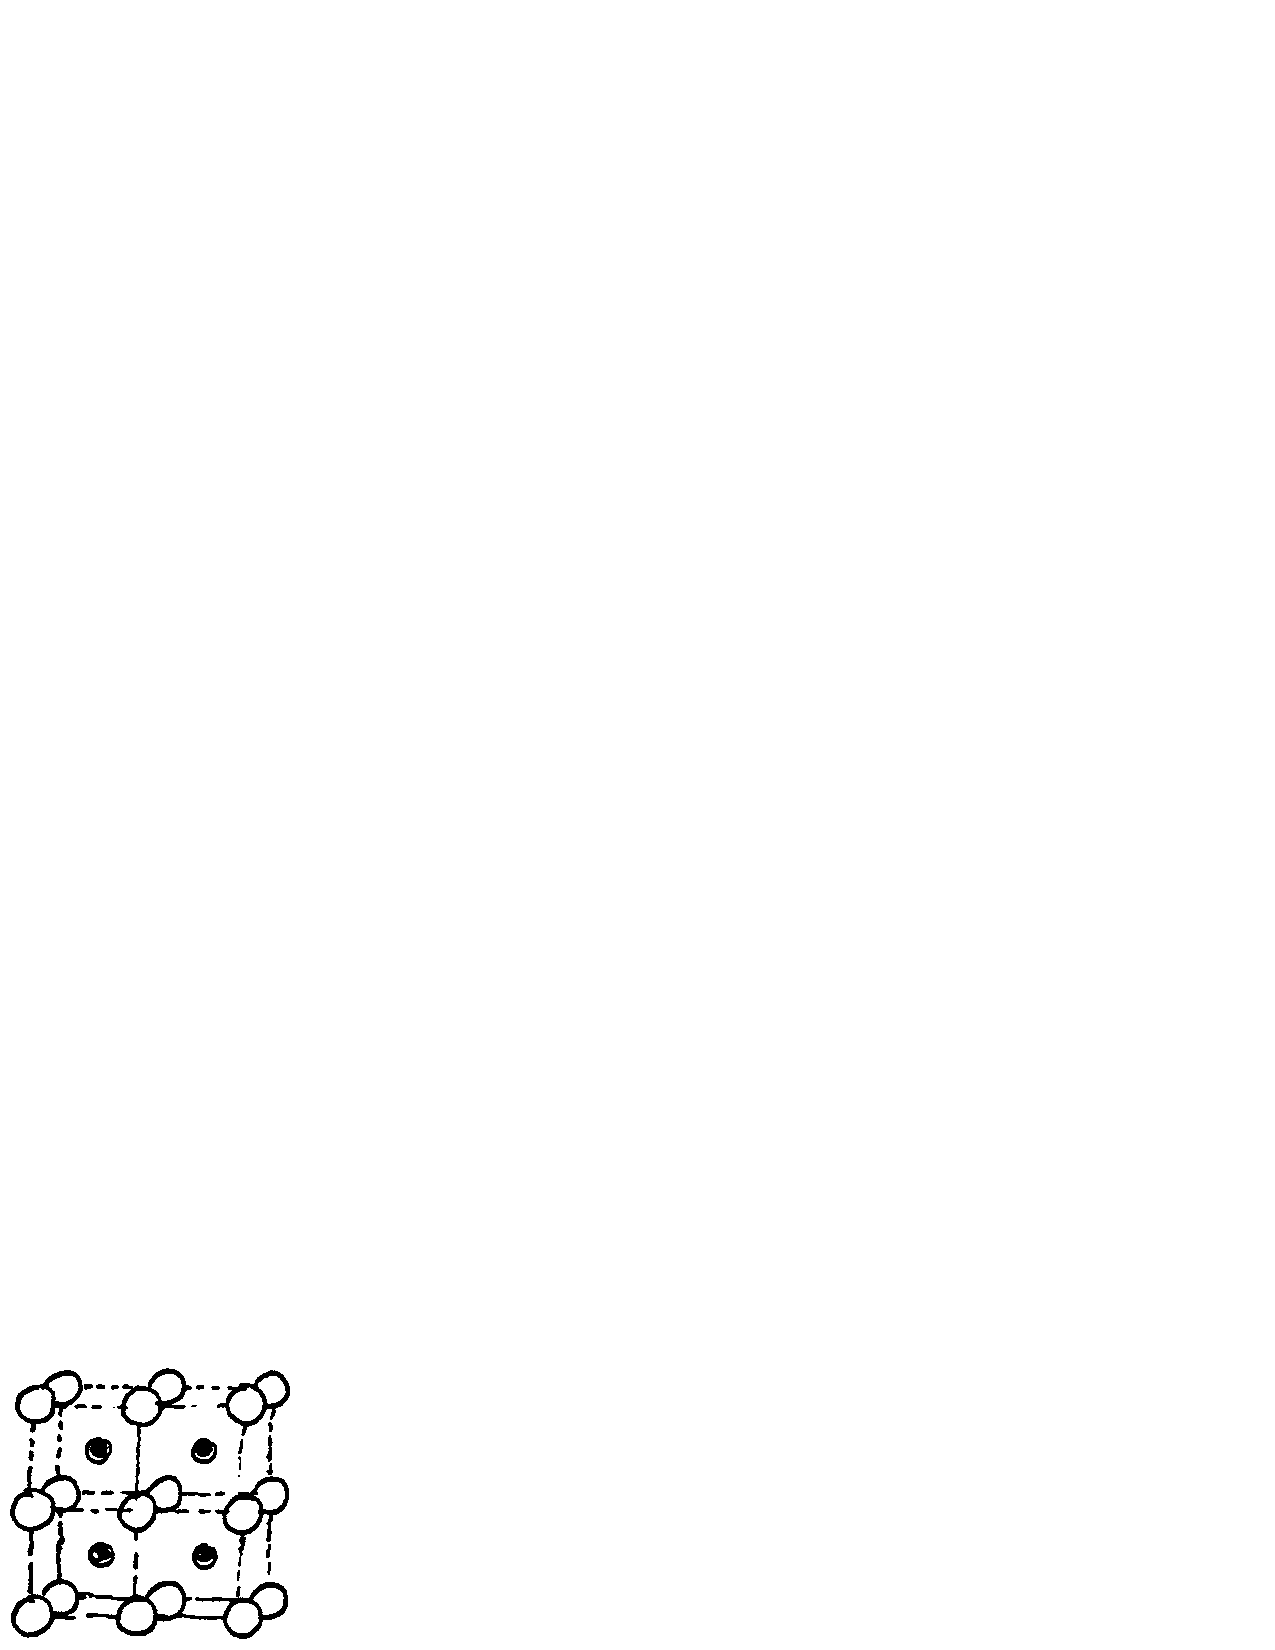
\includegraphics[scale=0.75]{fg9-06}
\caption{The CsCl structure, B2.}
\label{chap9-fig6}
\end{figure}

Crystal structures are generally referred to by the name of a prototype
molecule, exhibiting this structure, e.g., NaCl or CsCl, or by a numerical 
designation, e.g., B1 or B2, assigned by the review journal, 
Structure Reports or Strukturbericht, that first served the role of 
summarizing the results of various crystal structure determinations.

In Figure \ref{chap9-fig6}, starting with a cubic unit cell of length
$a$, one Cs is placed at the center of each cube, $({1 \over 2} a, {1
\over 2} a, {1 \over 2}a)$, and one Cl is placed at the corner,
(0,0,0).  The CsCl bond distance is ${1 \over 2} \sqrt{3} a$.  Each Cs
has eight Cl neighbors, and vice versa. The drawing contains four
cubic unit cells.

\begin{table}
\caption{}
\label{chap9-tab10}
\begin{tabular}{cccc}\\ \hline
& CN & R\cr

Na$^+$ & 4 & 0.990 & $-$3\% \cr
& 5 & 1.000 & $-$2\% \cr
& 6 & 1.020 & 0\cr
& 7 & 1.120 & +10\% \cr
& 8 & 1.180 & 16\% \cr
& 9 & 1.240 & 22\% \cr
& 12 & 1.390 & 37\% \cr
Mg$^{2+}$ & 4 & 0.570 & $-$21\% \cr
& 5 & 0.660 & $-$7\% \cr
& 6 & 0.720 & 0\cr
& 8 & 0.89 & +21\% \cr
Al${^3+}$ & 4 & 0.390 & $-$27\% \cr
& 5 & 0.480 & $-$10\% \cr
& 6 & 0.535 & 0\cr
Ti$^{4+}$ & 4 & 0.420 & $-$31\% \cr
& 5 & 0.510 & $-$16\% \cr
& 6 & 0.605 & 0\cr
& 8 & 0.740 & +22\% \cr
\hline
\end{tabular}
\end{table}

There is not yet a good real understanding of the fundamental reasons
why some compounds exhibit one crystal structure and others exhibit a
different structure.  However, for ionic crystals a consideration of
ion sizes provides a useful qualitative guide.  Assuming that each ion
is spherical and that the shortest bond distance is the sum of the two
ionic radii leads to the effective ionic radii in Table
\ref{chap9-tab10}.  Actually, the values in Table \ref{chap9-tab10}
were obtained with the restriction that $R(O^{2-})$ = 1.40 \AA.  This
somewhat arbitrary assumption is based on the distances between anions
for systems with very small cations.  A completely unconstrained fit
leads to anions that are 0.14 \AA\ smaller and cations that are 0.14
\AA\ larger.

\begin{figure}
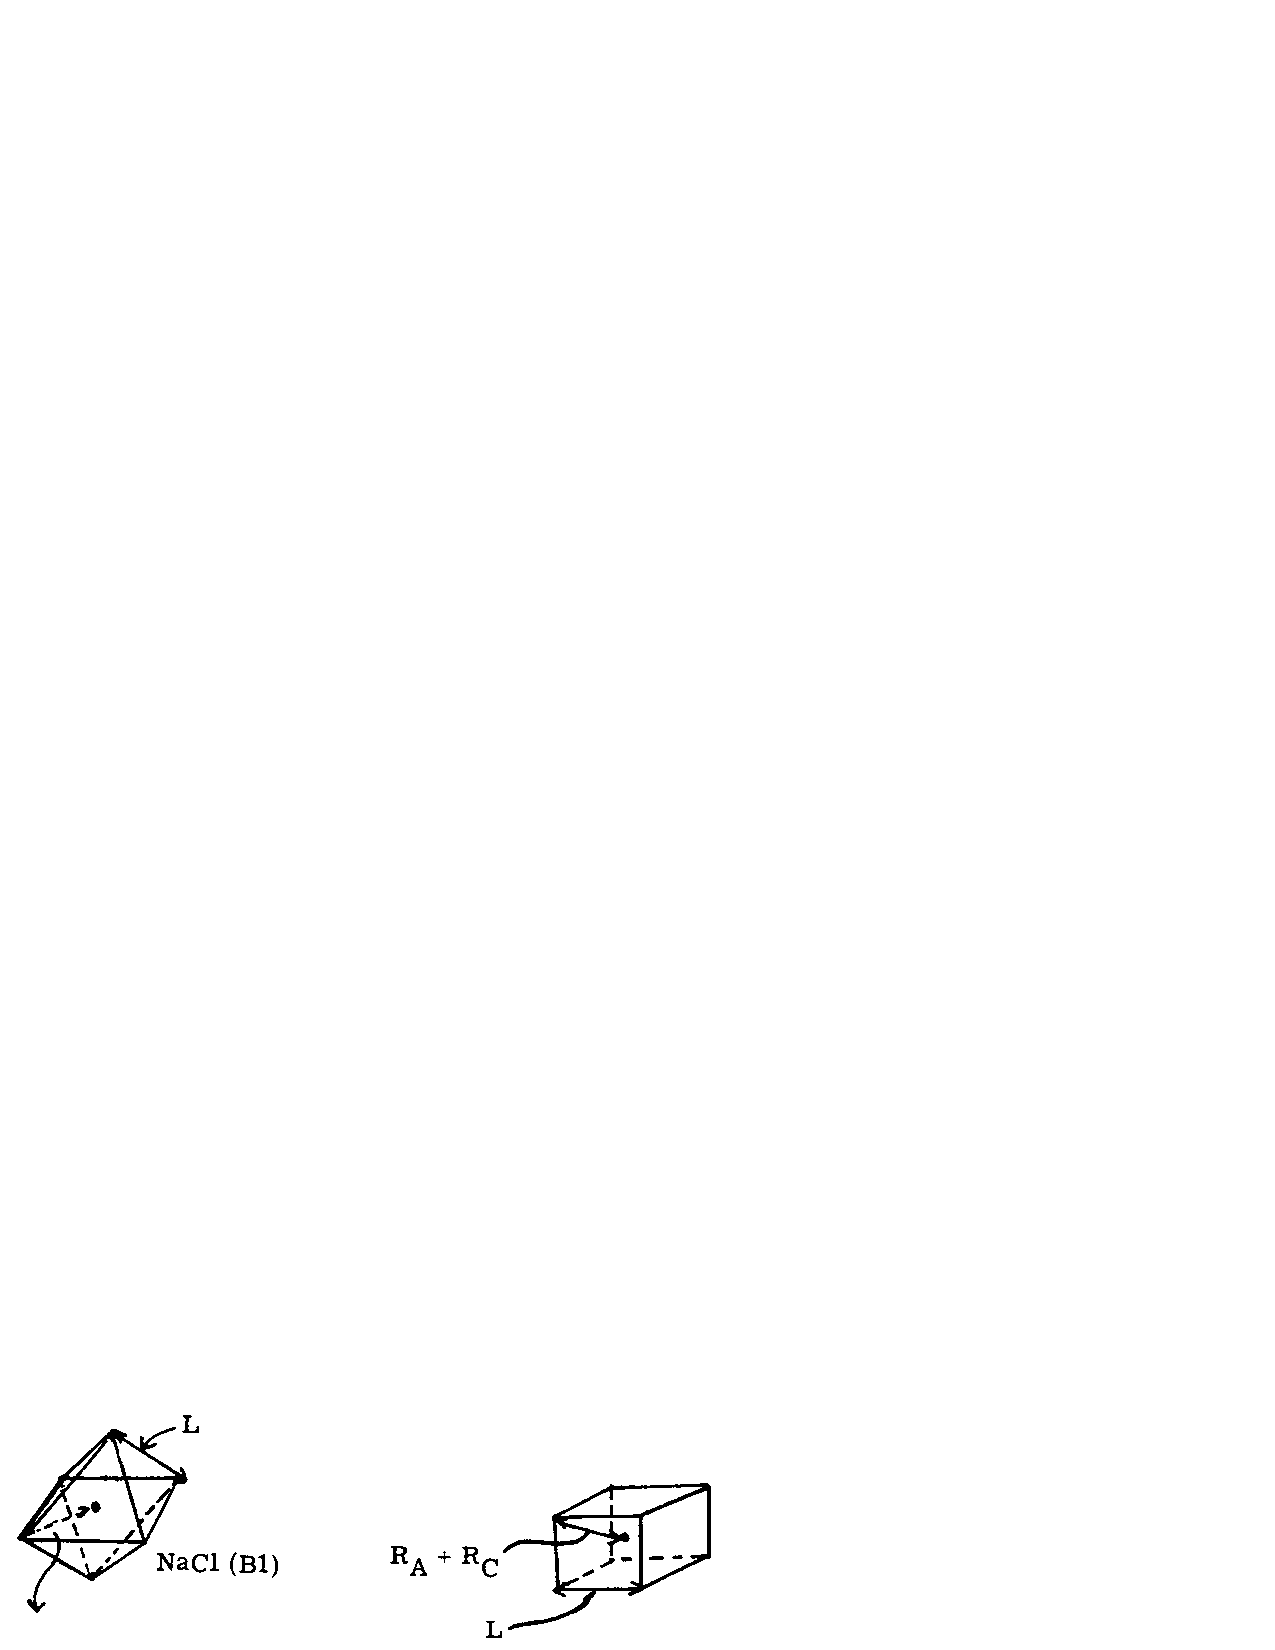
\includegraphics[scale=0.75]{fg9-07}
\caption{}
\label{chap9-fig7}
\end{figure}

In order to see how relative ion sizes might affect the choice of crystal 
structure, we will assume that the anions are in contact and calculate 
how big the hole is that is left for the cation.  For the B1 or NaCl 
structure, the cation is at the center of an octahedron of anions
(see Figure \ref{chap9-fig7})
so that $(R_A + R_C)/L = V1/\sqrt{2}$.  Since $2R_A < L = 
\sqrt{2}(R_A + R_C)$, we see that $R_C > 0.414 R_A$.  If the cation is 
any smaller than this, we cannot have the cation and anion
touching without having the anions overlap each other.  Consequently, the 
NaCl structure should be stable for
$$
{R_C \over R_A} \geq 0.414 .
\label{chap9-eqno14}
$$
For the CsCl structure, the same analysis leads to $(R_A + R_C)/L = 
\sqrt{3}/2$, so that $L \geq 2R_A$ leads to
$$
{R_C \over R_A} \geq 0.732 .
\label{chap9-eqno15}
$$
Consequently, for $0.414 \leq R_C/R_A \leq 0.723$, we expect the NaCl 
structure.  For $R_C /R_A < 0.414$ 
we expect some other structure to be favored, vide infra, while for
$R_C / R_A > 0.732$ either CsCl or NaCl is allowed.

\begin{table}
\caption{Radius ratios for alkali halides and noble metal 
halides.  The ionic radius is given adjacent to each ion.  Next to the radius 
ratio is the observed structure, B1, B2, B3, or B4.  Below the radius ratio 
is the difference between the observed and predicted bond distance for the BI 
structure.$^a$}
\label{chap9-tab11}
\begin{tabular}{cccccc}\\ \hline

& & F$^-$ & C$^-$ & Br$^-$ & I$^-$\cr
& & 1.33 & 1.81 & 1.96 & 2.20\cr

Li$^+$ & 0.76 & 0.57 B1 & 0.42 B1 & 0.39 B1 & 0.35 B1\cr
& & $-$0.08 & +0.01 & +0.03 & +0.04\cr
Na$^+$ & 1.02 & 0.77 B1 & 0.56 B1 & 0.52 B1 & 0.46 B1\cr
& & $-$0.04 & $-$0.01 & +0.01 & +0.02\cr
K$^+$ & 1.38 & 1.04 B1 & 0.76 B1 & 0.70 B1 & 0.63 B1\cr
& & $-$0.04 & $-$0.04 & $-$0.04 & $-$0.05\cr
Rb$^+$ & 1.52 & 1.14 B1 & 0.84 B1 (B2) & 0.78 B1 & 0.69 B1\cr
& & $-$0.01 & $-$0.04 & $-$0.05 & +0.05\cr
Cs$^+$ & 1.67 & 1.26 B1 & 0.92 B2 (B1) & 0.85 B2 & 0.76 B2\cr
& & 0.00 & +0.02\cr
Fr$^+$ & 1.94 & 1.46 & 1.07 & 0.99  & 0.88\cr
Cu$^+$ & 0.77 & 0.58 & 0.43 B4 & 0.39 B4 & 0.35 B4\cr
Ag$^+$ & 1.15 & 0.86 B1 & 0.64 B1 & 0.59 B1 & 0.52 B3, B4\cr
Au$^+$ & 1.37 & 1.03 & 0.76 & 0.70 & 0.62 Tet\cr
\hline
\end{tabular}\\
$^a$ Based on R. W. G. Wyckoff, Crystal Structures Second Edition, 
Volume 1, 1963.
\end{table}

In Table \ref{chap9-tab11} we indicate the stable structures and
radius cations for a number of ionic molecules.  Here, we see that the
radius ratio for the B1 or NaCl structure is 0.35 to 1.26, while the
radius ratio for the CsCl structure is 0.76 to 0.92.  Thus, the
observed structures are in reasonable agreement with the criteria in
(\ref{chap9-eqno14}) and (\ref{chap9-eqno15}).  However, the analysis
does not explain which structure should be observed for $R_C / R_A >$
0.73.

\subsubsection{Coordination Dependence of Ion Sizes}

Although the B2 structure is the stable one for CsCl, it can also be 
prepared in the B1 structure.  However, the CsCl bond distances in 
these structures are different:
\smallskip
\centerline{B1: $R_{CsCl} =$ 3.51\AA}
\centerline{B2: $R_{CsCl} +$ 3.57\AA}
\smallskip

\noindent
This is typical, the effective size of an ion increases as its
coordination number increases.  The values in Table \ref{chap9-tab10}
are for a coordination number of 6 and must be modified for other
cases.  Typical corrections are given in Table \ref{chap9-tab10},
where we see that the effects are significant and increase as the
charge increases.

\subsection{Divalent Ionic Structures}

For the divalent ionic crystals MX where X$^{2-} =$ O, S, Se, or Te
and M$^{2+}$ = Be, Mg, Ca, Sr, Ba, Zn, Cd, or Hg, we also include Mn
since the Mn$^{++}$ ion is a spherically symmetric $d^5$
configuration, the cations lead to small radius ratios, in some cases
much smaller than 0.4.  As a result, some MX cases lead to structures
in which M is tetrahedrally coordinated, as in Figures
\ref{chap9-fig8} and \ref{chap9-fig9}.


\begin{figure}
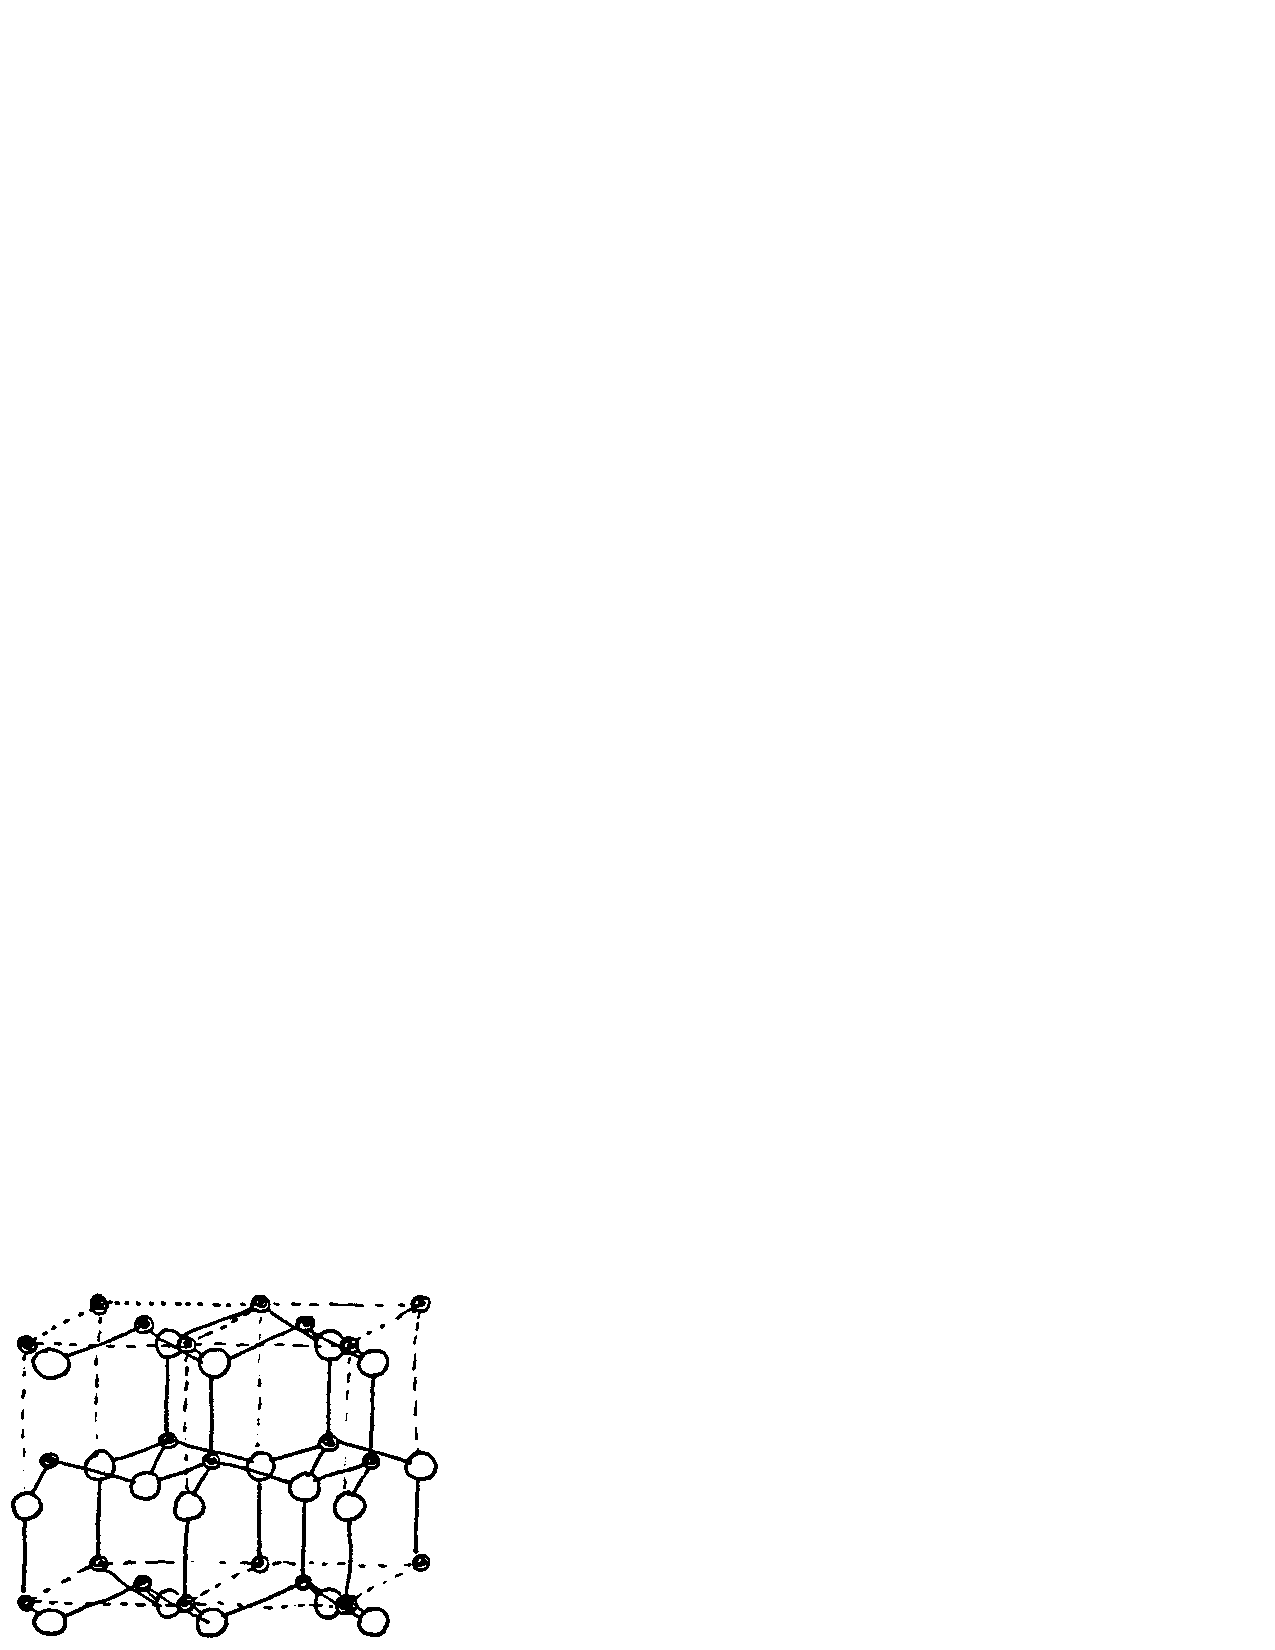
\includegraphics[scale=0.75]{fg9-08}
\caption{The Wurtzite (ZnS), or zincite (ZnO) 
structure (B4). Each Zn is in a tetrahedron of O, and each O has four
Zn nearest neighbors.  The O, and Zn, are each in an hexagonal
closest-packed arrangement.  At each atom, there is threefold symmetry
about the z axis. The dashed lines outline the orthogonal unit cell
with a $L_x/L_y = \sqrt{3}$.}
\label{chap9-fig8}
\end{figure}

\begin{figure}
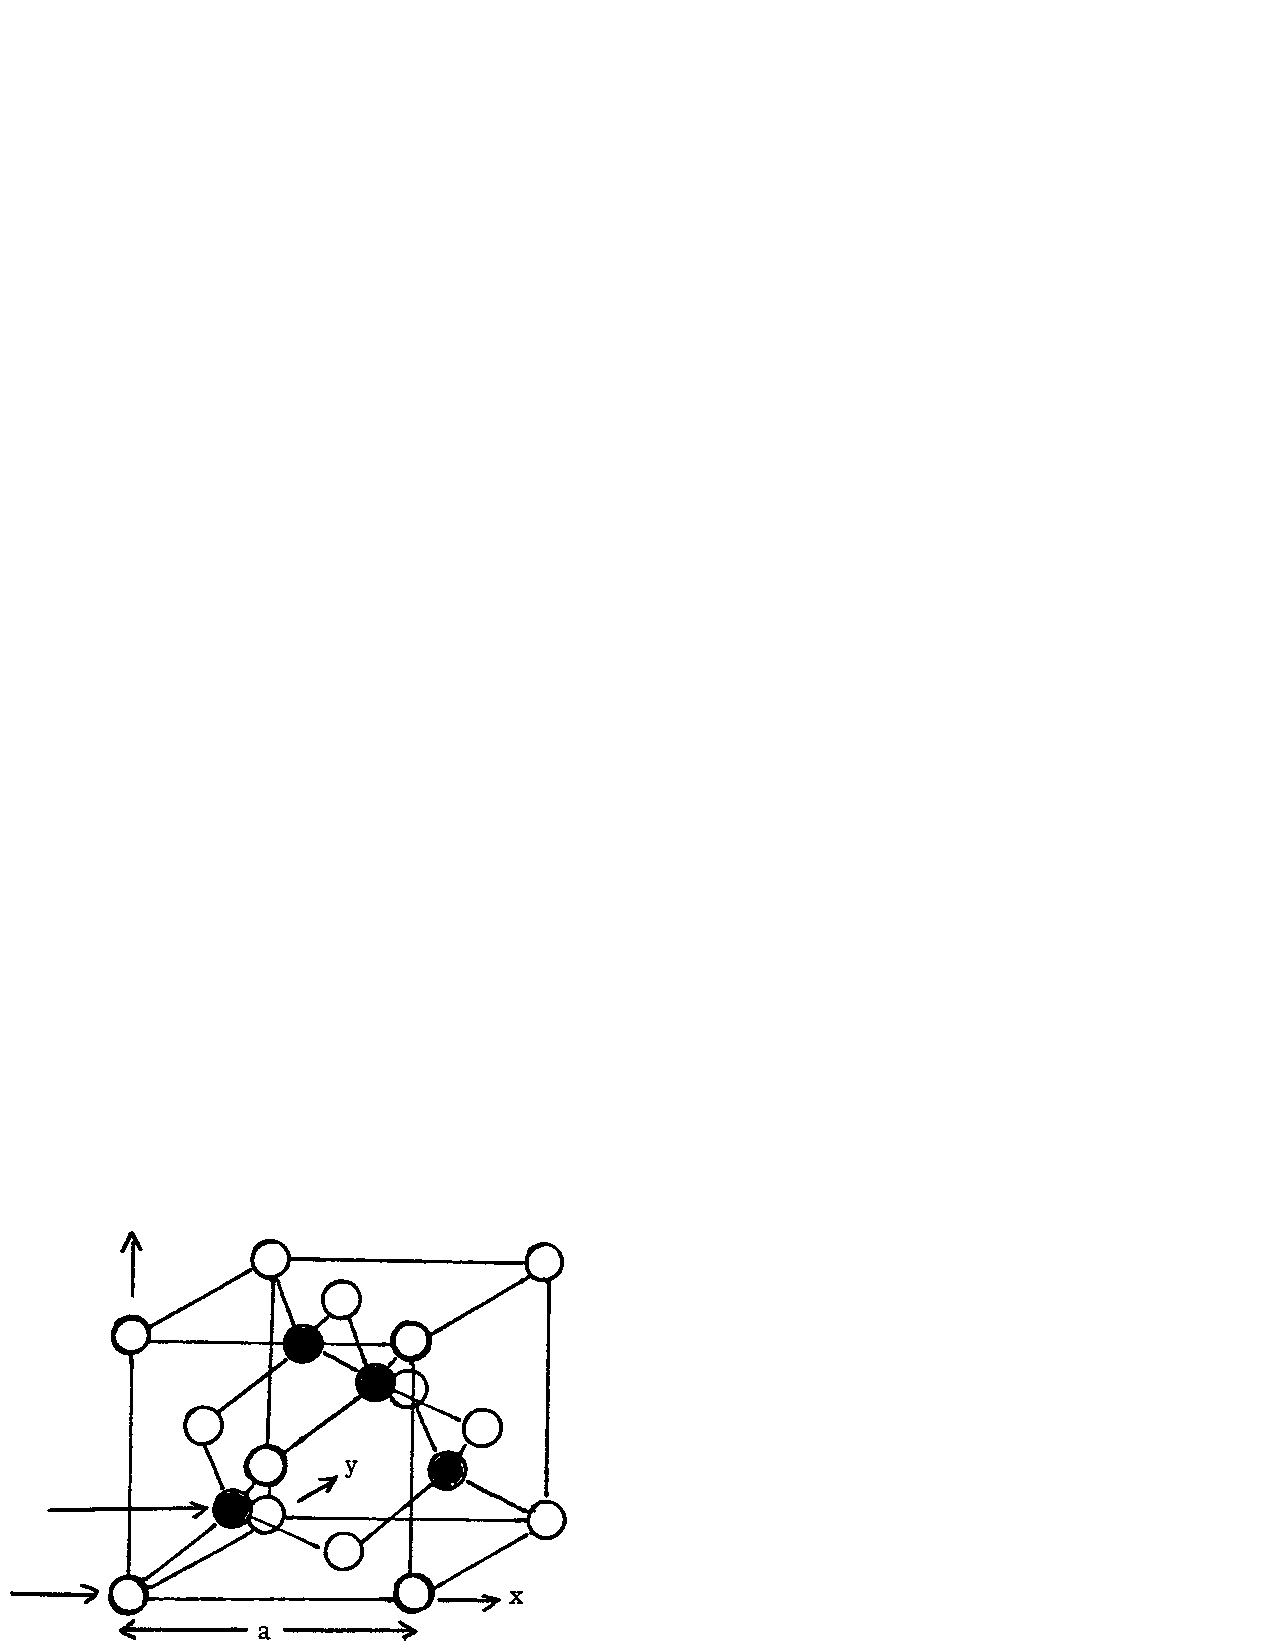
\includegraphics[scale=0.75]{fg9-09}
\caption{The sphalerite or zincblende (ZnS) 
structure (B3). This is identical to
diamond except that two types of atoms are present.  Each
Zn is in a tetrahedron of S and each S has four Zn nearest neighbors. If
$a$ is the size of the cubic unit cell, there are Zn at $({1 \over 
4}a, {1 \over 4} a, {1 \over 4}a)$, (${3 \over 4} a, {3 \over 4}a , 
{1 \over 4} a)$, $({1 \over 4} a , {3 \over 4} a , {3 \over 4} a)$, 
and $({3 \over 4} a, {1 \over 4} a, {3 \over 4} a)$, and S at the 
corners (0,0,0), and face centers $(0 , {1 \over 2} a , {1 \over 2} 
a)$, $({1 \over 2} a , 0 , {1 \over 2} a)$, and $({1 \over 2} a , {1 
\over 2} a , 0)$.  The S, and Zn, are each in a
cubic closest-packed arrangement.}
\label{chap9-fig9}
\end{figure}

\begin{figure}
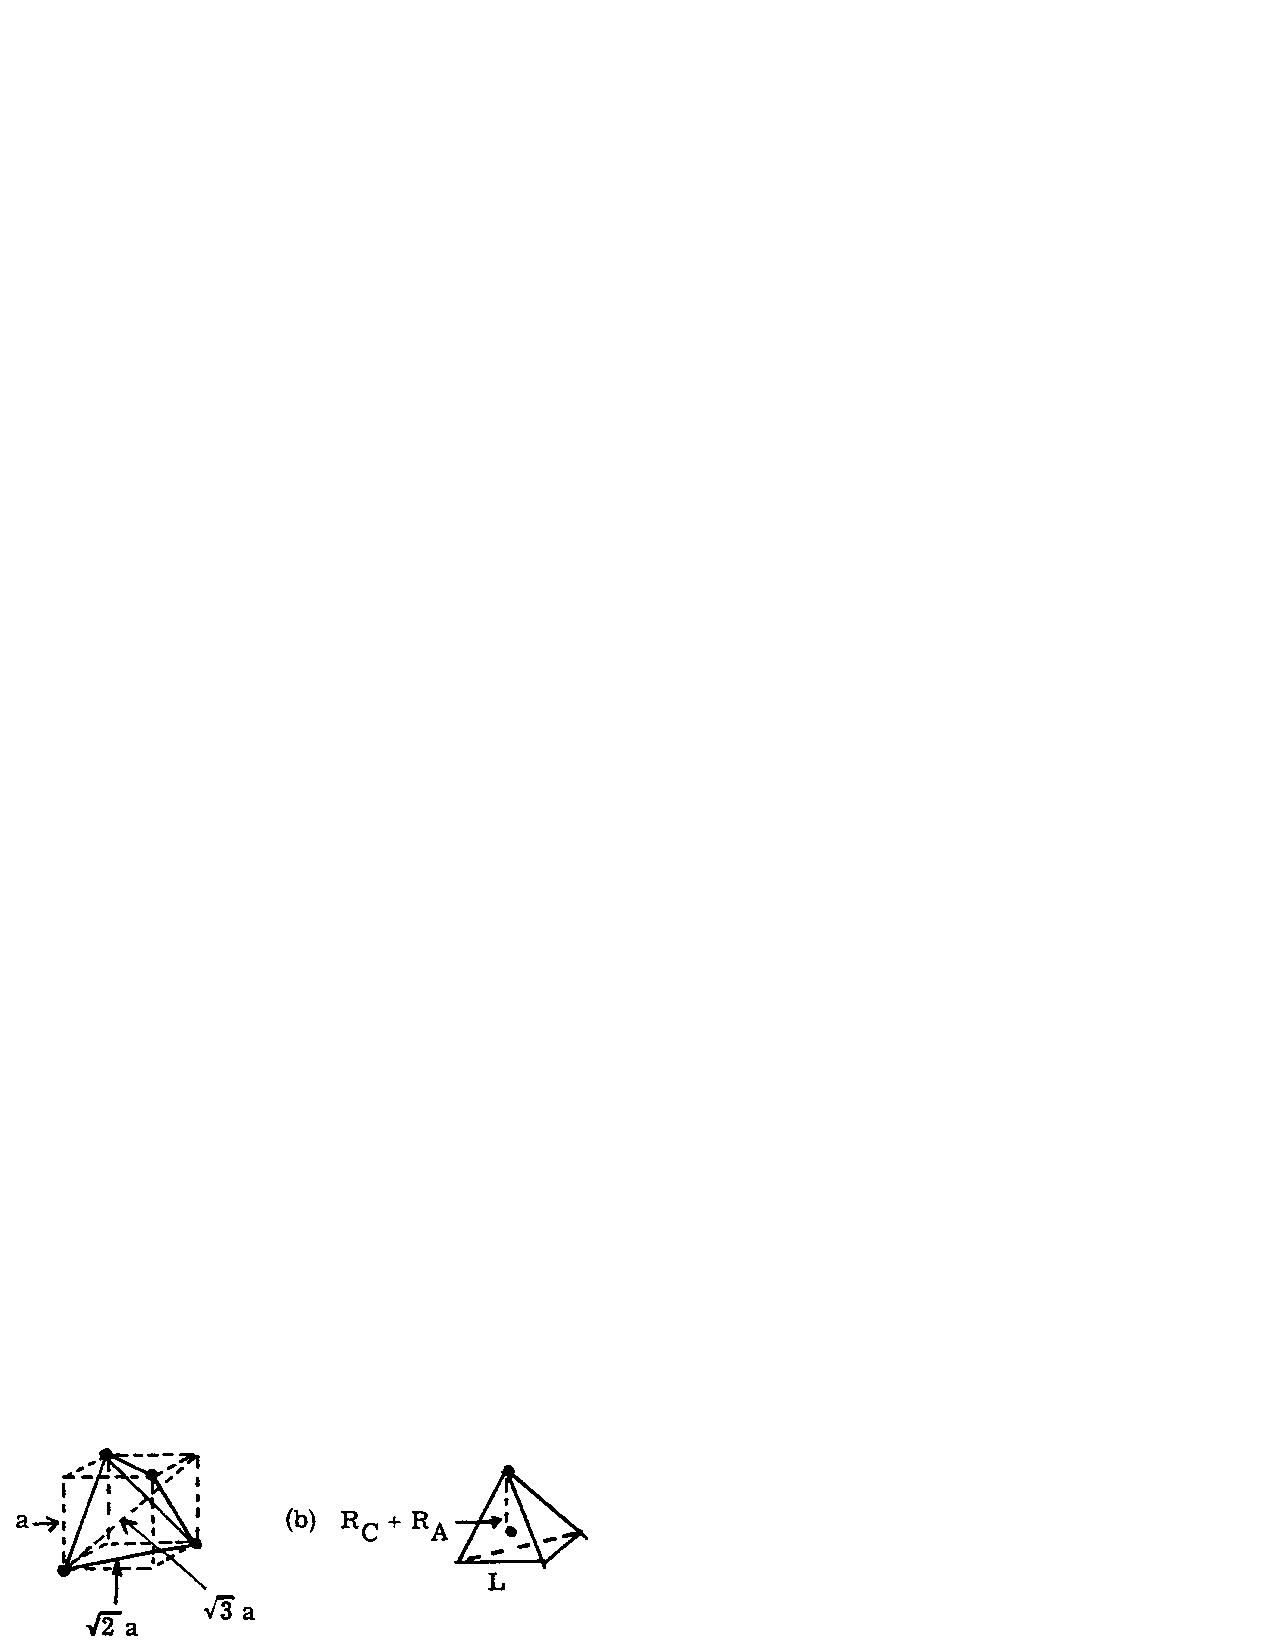
\includegraphics[scale=0.75]{fg9-10}
\caption{}
\label{chap9-fig10}
\end{figure}

As is clear in Figure \ref{chap9-fig10}(a), the height of a
tetrahedron is $2/3\sqrt{3}a$, where $a$ is the side of the
circumscribed cube.  Therefore, the midpoint of the tetrahedron, also
the midpoint of the cube, is $1/2 \sqrt{3}a$ from the vertex, and
hence, from Figure \ref{chap9-fig10}(b)
$$
{R_C + R_A \over L} = {{1 \over 2} \sqrt{3}a \over \sqrt{2}a} = 
\sqrt{{3 \over 8}} = 0.612.
$$
Thus,
$$
2R_A < L = \sqrt{{3 \over 8}} \left( R_C + R_A \right) = 1.633 \left( 
R_C + R_A \right) 
$$
or $1.225 R_A < R_C + R_A$ or $R_C / R_A > 0.225$.  Thus, in the range
$0.225 < R_C / R_A < 0.414$, the B4 and B3 structures with tetrahedral 
coordination should be stable.

As indicated in Table \ref{chap9-tab12}, the overall trends are
basically in agreement with these expectations, with B4 and B3
observed for $0.20 < R_C / R_A < 0.55$ and B1 observed for $0.36 < R_C
/ R_A < 0.96$.

\begin{table}
\caption{Radius ratios and observed structures for 
divalent XY systems.  The ionic radius is given next to each ion.$^a$}
\label{chap9-tab12}
\begin{tabular}{cccccc}\\ \hline
& & O$^-$ & S$^-$ & Se$^-$ & Te$^-$\cr
& & 1.40 & 1.84 & 1.98 & 2.21\cr

Be & 0.45 & 0.32 B4 & 0.24 B3 & 0.23 B3 & 0.20 B3\cr
Mg & 0.72 & 0.51 B1 & 0.39 B1 & 0.36 B1 & 0.33 B4\cr
Ca & 1.00 & 0.71 B1	& 0.54 B1 & 0.51 B1	& 0.45 B1\cr
Sr & 1.18 & 0.84 B1	& 0.64 B1 & 0.60 B1	& 0.53 B1\cr
Ba & 1.35 & 0.96 B1	& 0.73 B1 & 0.68 B1 & 0.61 B1\cr
Zn & 0.74 & 0.53 B4	& 0.40 B3,4 & 0.37 B3,4 & 0.33 B3,4\cr
Cd & 0.95 & 0.68 B1	& 0.52 B3,4 & 0.48 B4 & 0.43 B3,4\cr
Hg & 1.02 & 0.73 & 0.55 B3 & 0.52 B3 & 0.46 B3\cr
Mn & 0.83 & 0.59 B1 & 0.45 B1,3,4 & 0.42 B1,3,4 & 0.38 B4\cr
\hline
\end{tabular}\\
$^a$ Based on Wyckoff, loc. cit.
\end{table}

\subsection{MX$_2$ Structures, Fluorite and Rutile}

A number of compounds have unqual numbers of cations and anions.  For
example, fluorite, CaF$_2$, has the structure in Figure
\ref{chap9-fig11}, in which the anions are arranged in a simple cubic
array, and Ca occupies alternate sites at the center of the cubes.

\begin{figure}
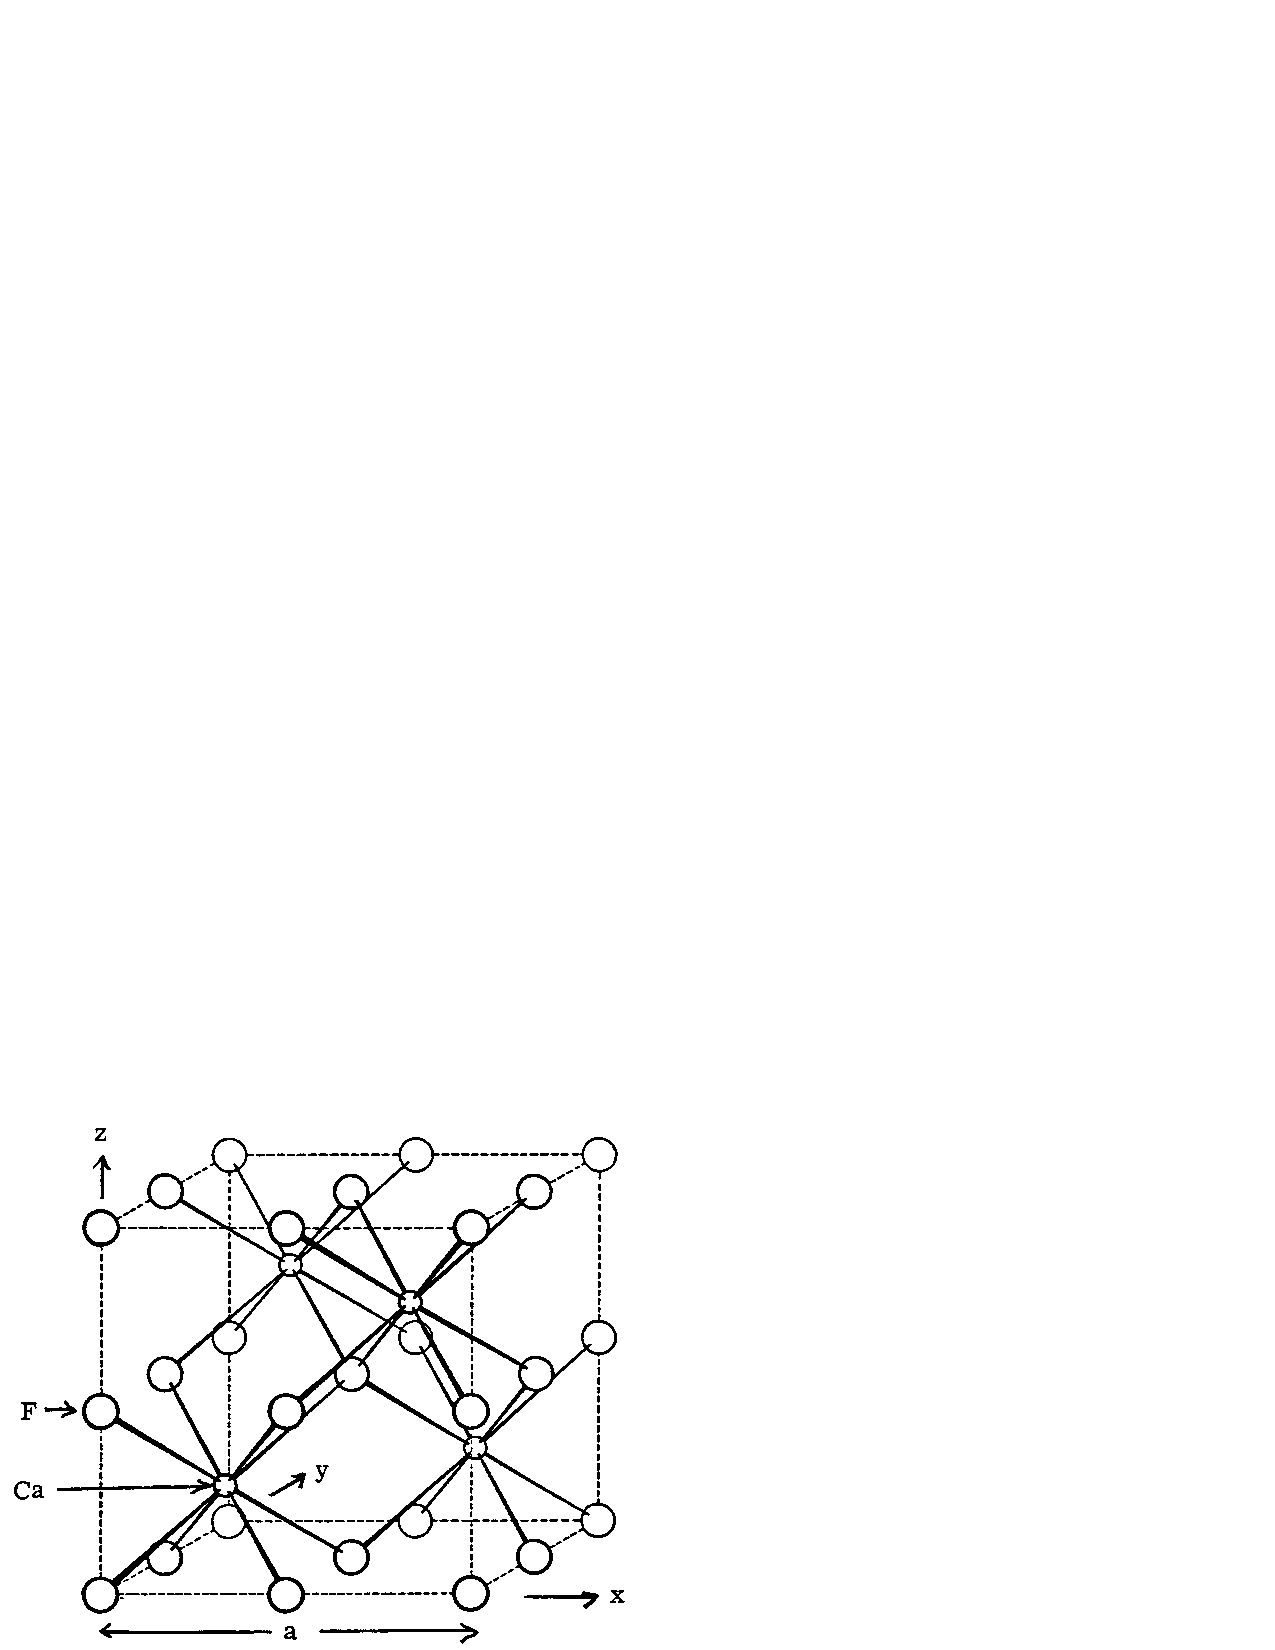
\includegraphics[scale=0.75]{fg9-11}
\caption{The structure of the cubic crystal fluorite, 
CaF$_2$.  Small circles represent calcium ions and large circles fluoride 
ions.  Using a cubic unit cell of side $a$, the Ca are at $({1 \over 
4} a , {1 \over 4} a , {1 \over 4} a)$, $({3 \over 4}a , {3 \over 4} 
a, {1 \over 4} a)$, $({3 \over 4} a , {1 \over 4} a , {3 \over 4} a)$, 
and $({1 \over 4} a, {3 \over 4} a , {3 \over 4} a)$, while the F are at 
the corners, centers of edges, centers of faces, and center of cube.  Each 
Ca is in a cube of F, and each F has four nearest neighbor Ca's.
}
\label{chap9-fig11}
\end{figure}

This is just like the CsCl structure but with half the Cs missing.
Another common structure is the rutile, TiO$_2$, or cassiterite,
SnO$_2$, crystal structure in Figure \ref{chap9-fig12}.

\begin{figure}
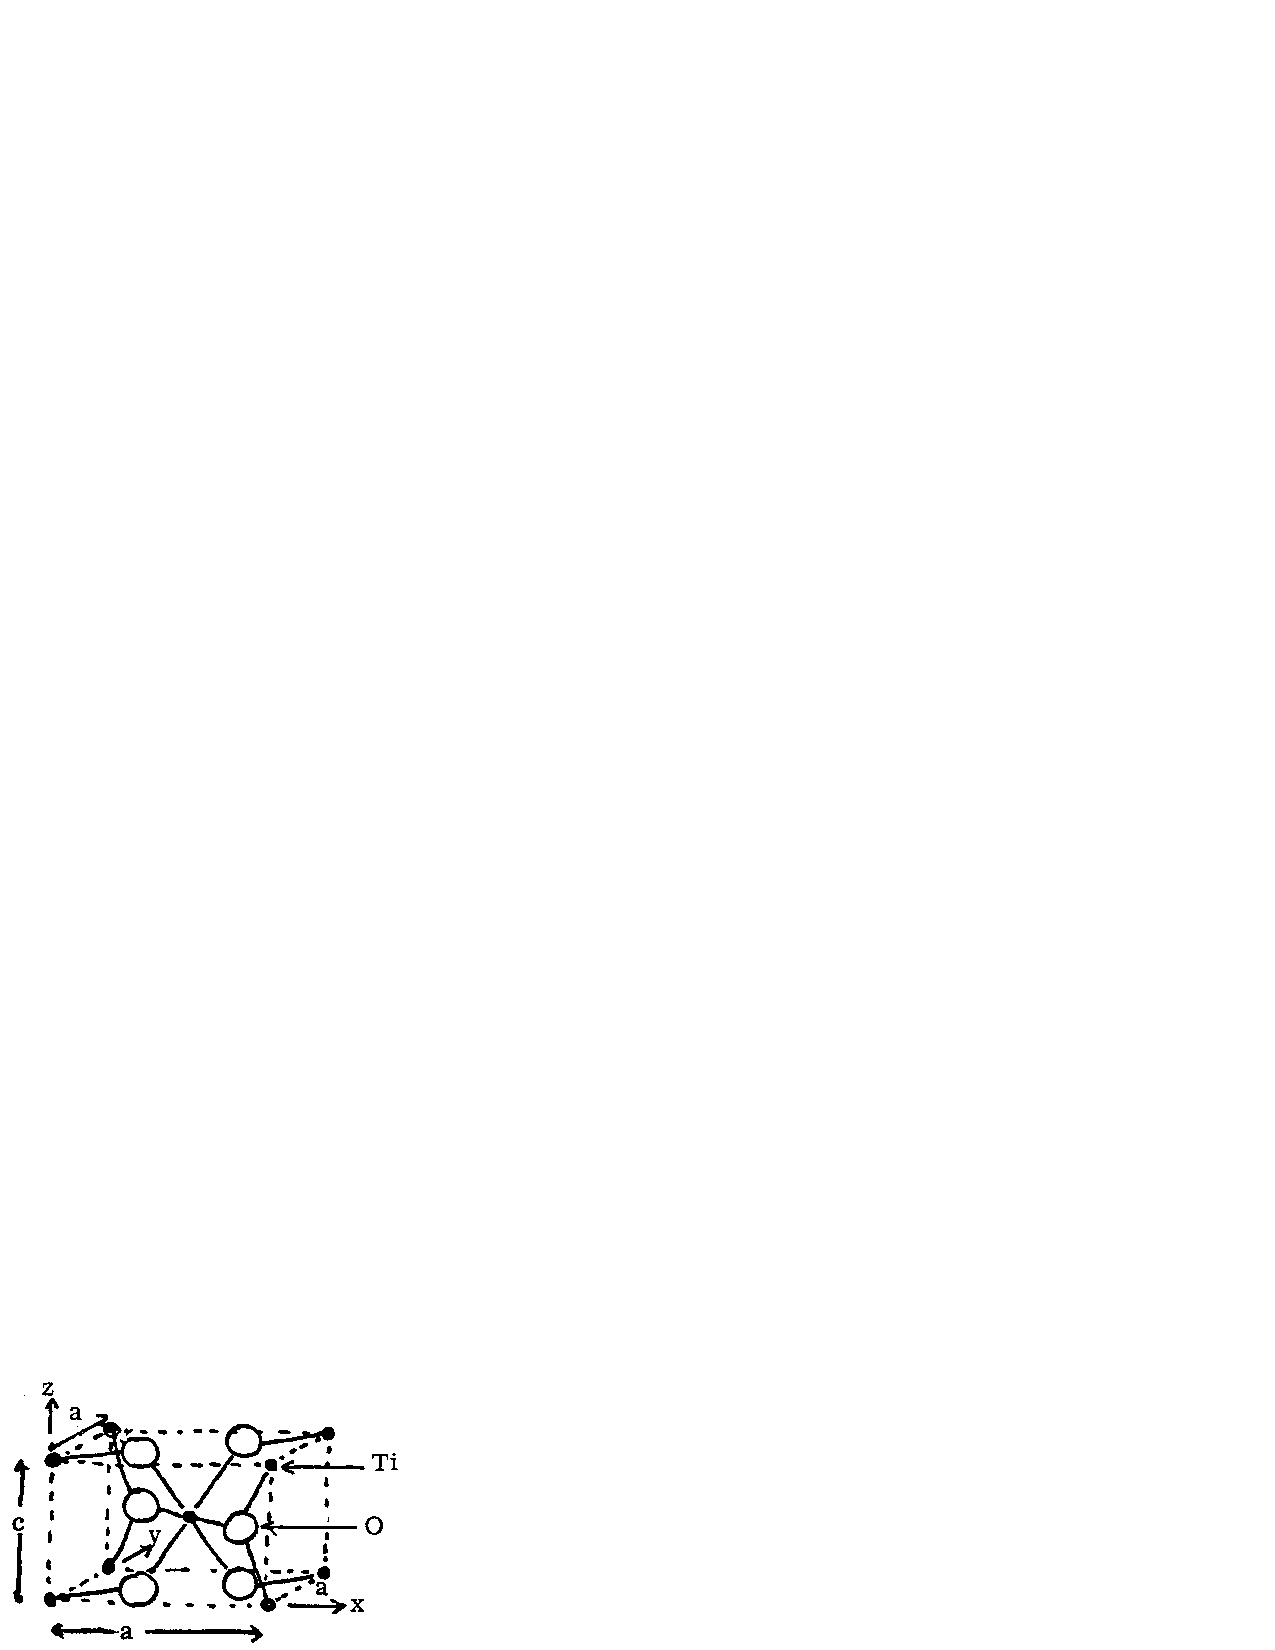
\includegraphics[scale=0.75]{fg9-12}
\caption{The unit cell for the rutile (TiO$_2$) or cassiterite 
(SnO$_2$) crystal structure.  Ti atoms are at the corners and center
of the unit cell, $(0,0,0)$, $({1 \over 2} a , {1 \over 2} a, {1 \over
2} a)$.  O atoms are in the $z = 0$, and $z = c$, planes at $({1
\over 4}a , {1 \over 4} a, 0)$ and $( {3 \over 4} a, {3 \over 4} a, 
0)$, and in the $x = c/2$ plane at $({1 \over 4} a, {3 \over 4} a, {1 
\over 2} c)$, and $({3 \over 4} a, {1 \over 4} a , {1 \over 2} c)$.  The 
full, distorted, octahedron of O for the central Ti is
shown.  Each O is coordinated to three Ti, all in the same plane, as is
clear for the two oxygens in the $z = 1/2c$ plane.}
\label{chap9-fig12}
\end{figure}


This is related to the NaCl structure, but with half of the cations
missing.  Just as with NaCl versus CsCl, the rutile structure prefers
smaller cations than does fluorite.  In Table \ref{chap9-tab13} we
list all known MX$_2$ and MO$_2$ cases of c these two structures.  For
MF$_2$ we see that rutile is always found for $R_C/R_A < 0.67$, while
fluorite is always found for $R_C/R_A > 0.71$, a result that is in
excellent agreement with the critical ratio of 0.73 in
(\ref{chap9-eqno15}).  For Cl the fluorite structure is observed
above, $R_C/R_A = 0.65$, still reasonably close to expectations.  For
MO$_2$ the dividing line is $R_C/R_A = 0.50$, if the questionable
structures RuO$_2$, PbO$_2$, and TeO$_2$ are excluded.  This is not in
good agreement with (\ref{chap9-eqno15}), suggesting that the O$^{2-}$
anions are not allowed to approach as close as $2R_A$.  These
correlations suggest that TeO$_2$ should not have the rutile
structure, and that RuO$_2$ and PbO$_2$ should be reexamined.

\begin{table}
\caption{Observed structures for MF$_2$ and MO$_2$ 
crystals.  Compounds above the solid line exhibit the rutile
crystal structure, while those below the line exhibit the fluorite crystal 
structure. (d) indicates a strongely distorted rutile structure, and ?
indicates that the data reported in the literature are old and without the
intensity analyses needed to prove structure.$^a$}
\label{chap9-tab13}
\begin{tabular}{cccc}\\ \hline

NiF$_2$ & 0.52 & GeO$_2$ & 0.38\cr
MgF$_2$ & 0.54 & $\beta$-MnO$_2$ & 0.38\cr
CuF$_2$ (d) & 0.55 & CrO$_2$ & 0.39\cr
ZnF$_2$	& 0.56 & VO$_2$ & 0.41\cr
FeF$_2$	& 0.59 & ReO$_2$ (d)$^b$ & 0.41\cr
MnF$_2$	& 0.62 & TiO$_2$ & 0.43\cr
PdF$_2$ {\rm (?)} & 0.65 & IrO$_2$ {\rm (?)} & 0.45\cr
CoF$_2$	& 0.67 & OsO$_2$ {\rm (?)} & 0.45\cr
& & TcO$_2$ (d)$^b$ & 0.46\cr
& & MoO$_2$ (d) & 0.46\cr
& & WO$_2$ (d) & 0.47\cr
& & NbO$_2$ (d) & 0.49\cr
& & TaO$_2$ & 0.49\cr
& & SnO$_2$ & 0.49\cr
& & RuO$_2$ {\rm (?)} & 0.54\cr
& & PbO$_2$ & 0.55\cr
& & TeO$_2$ & 0.69\cr

CdF$_2$ & 0.71 & HfO$_2$ & 0.51\cr
SrCl$_2$ & 0.65 & ZrO$_2$ & 0.51\cr
BaCl$_2$ & 0.75	& TbO$_2$ &	0.54\cr
CaF$_2$ & 0.75 & AmO$_2$ & 0.61\cr
EuF$_2$ & 0.88 & CmO$_2$ & 0.61\cr
SrF$_2$ & 0.89 & PrO$_2$ & 0.61\cr
HgF$_2$ & 0.89 & PuO$_2$ & 0.61\cr
BaF$_2$ & 1.02 & CeO$_2$ & 0.62\cr
RaF$_2$ & 1.08 & NpO$_2$ & 0.62\cr
& & UO$_2$ & 0.64\cr
& & PaO$_2$ & 0.64\cr
& & $\alpha$-PoO$_2$ & 0.67\cr
& & ThO$_2$ & 0.67\cr
\hline
\end{tabular}\\
$^a$ Unless stated otherwise, data from Wyckoff, loc. cit.
$^b$ W. A. Goddard III.
\end{table}

\subsection{More Complex Ionic Crystals}

In silica, SiO$_2$, each Si has four oxygen neighbors.  Assuming Si is
Si$^{4+}$, then each bond involves a charge transfer of +1.  This
charge must come from the O, and since each O is O$^{2-}$, then each O
must be coordinated to two Si. This type of reasoning is generally
useful in ascertaining the structures of ionic crystals.  The general
rule is: the electrostatic balance postulate.  If $+z_ce$ is the total
electronic charge of a cation and $\nu_c$ is its coordination number,
then the polarity, S, of each electrostatic bond to this cation is $S=
z_c/\nu_c$.  Letting the charge of the anion be $-z_ae$, then the sum
of the bond polarities involving this anion must be
$$
z_a = \sum_{i} S_i = \sum_{i} {z_{ci} \over \nu_i},
$$
where the sum is over all cations at the centers of polyhedra involving the 
given anion.

As examples of this rule, consider the following minerals:
\begin{enumerate}
\item Silica, SiO$_2$. As indicated above, each Si is in a 
tetrahedron of O$^=$ anions, leading to S = 1.  Thus, each O$^=$ must 
have just two Si neighbors. Consequently, the structures of silica
can be constructed by putting together tetrahedra where each corner 
connects exactly two tetrahedra.

\item Rutile, Anatase, and Brookite, TiO$_2$.  The Ti$^{4+}$ 
is in a distorted octahedron of O$^=$ anions.  Since the bond polarity is 
S = 4/6, each O$^=$ must be coordinated to three Ti$^{4+}$ centers.
This structure for rutile is illustrated in Figure \ref{chap9-fig3}.

\item Corundum, Al$_2$0$_3$. The Al$^{3+}$ is in a distorted 
octahedron of O$^=$ anions. Since the
bond polarity is S = 3/6, each O$^=$ must be coordinated to four 
Al$^{3+}$ centers.

\item Olivine, Mg$_2$SiO$_4$.  Each Si has four O$^=$ neighbors, S = 
1, and each Mg has six, S = 1/3. Thus, each O$^=$ must have one Si and 
three Mg neighbors.

\item Aluminosilicates.  Both the Al$^{3+}$ and Si$^{4+}$ are at the 
centers of O$^=$ tetrahedra and the tetrahedra are connected as in silica, 
with each corner connecting two tetrahedra.  Two tetrahedra containing Al 
are never connected; thus, the choices are to connect two Si
tetrahedra or else one Al and one Si tetrahedron.  In this latter case, the 
total bond polarity to the bridging 0 is only 1 + 3/4 = 7/4.  In order to 
obtain a balance of charge, the various minerals incorporate large 
monovalent ions such as K$^+$ or Na$^+$, or large divalent ions such as 
Ca$^{++}$ or Ba$^{++}$. In either case, these extra cations must 
have S = 1/4 so that K$^+$ or Na$^+$ should have four O$^=$ near 
neighbors, while Ca$^{++}$ or Ba$^{++}$ should have eight, if
exact electrostatic balance is to be maintained.  Examples include, feldspars 
such as albite, NaAlSi$_3$O$_8$; orthoclase, KAlSi$_3$O$_8$; celsian, 
BaAl$_2$Si$_2$O$_8$; and, anorthite, CaAl$_2$Si$_2$O$_8$, 
that are essential constituents of nearly all crystalline 
rocks, e.g., granite, gneis, most basalts, and trachyte. Notice that the 
total number of Al and Si is just half the total number of 0 anions.
\end{enumerate}

As discussed above, the silicate tetrahedra of silica and various silicates 
are connected so that each O connects two tetrahedra.  This could be done 
in three ways:
\begin{enumerate}
\item Sharing corners:
\begin{equation}
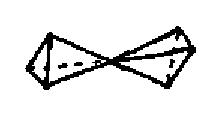
\includegraphics{fg9-12a-1}
\end{equation}
\item Sharing edges:
\begin{equation}
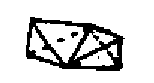
\includegraphics{fg9-12a-2}
\end{equation}
\item Sharing faces:
\begin{equation}
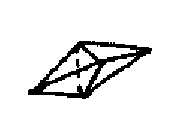
\includegraphics{fg9-12a-3}
\end{equation}
\end{enumerate}
The distances between the centers for these cases are 1, 0.58, and 0.33, 
respectively, so that the latter two cases would have very short 
cation-cation distances.  Indeed, such tetrahedra are nearly always 
connected by sharing corners, no exceptions are known for Si.

Similarly, octahedra, e.g., AlO$_6$ or TiO$_6$, may be connected by
sharing corners, edges, or faces.  In this case, the distances between
centers are 1, 0.71, and 0.58.  This is less severe than for
tetrahedra and many cases are known where octahedra share edges, and
some examples exist where faces are shared.  For example, in rutile,
each octahedron shares two edges with adjacent octahedra, see Figure
\ref{chap9-fig12}.

\subsection{Use of the Electrostatic Balance Postulate}

See problem number two of the Exercise section.  A structure with
TiO$_6$, orbitals and N$_{Ti} = 2$ is easy to construct.  Put Ti at
the center of a cube and O at the centers of faces, as in Figure
\ref{chap9-fig13}.

\begin{figure}
% Warning: figure missing from ch9 p 31
%\includegraphics[scale=0.75]{fg9-}
\caption{The structure of perovskite (CaTiO$_3$) or BaTiO$_3$.
Ti is a small circle, O is a large circle, and Ca or Ba is a cross.}
\label{chap9-fig13}
\end{figure}

Each Ti has six equidistant oxygen neighbors in an octahedral
arrangement.  Each O has just two Ti neighbors, centers of adjacent
cubes. The total number of Ti in the cube is 1, and the total number
of O in the cube is $6 \times 1/2 = 3$ atoms, since each face is
shared by two cubes.  Thus, the composition is TiO$_3$, and we need to
find a place for the Ba.  An alternative view of this structure is
given in Figure \ref{chap9-fig13}(b), where the cube has shifted so
that Ti is at the corners. This still leads to TiO$_3$ as the
composition since one Ti at each corner accounts for $8 \times 1/8 =
1$ atom, since each corner is shared by eight cubes, and the O at each
edge accounts for $12 \times 1/4 = 3$ atoms, since each edge is shared
by four cubes.  The case of N$_{Ba} = 4$ or $\nu_{Ba} = 12$ is easy.
Put the Ba at the center of the cube in Figure \ref{chap9-fig13}b.
This has twelve nearest neighbor O's, and each O has four nearest
neighbor Ba's, the center of the four cubes shared by the edge.
Assuming that the oxygens are in contact, the space available for the
Ti$^{++}$ is
$$
{R_{Ti} + R_O \over 2R_O} = {1 \over \sqrt{2}}
$$
or $R_{Ti} =$ 0.414 $R_O =$ 0.58\AA, in reasonable agreement with the
size of Ti$^{4+}$, 0.605 \AA.  The space available, diameter, for the
Ba at the center of the cube is $\sqrt{2}a - 2R_O - 2R_O = 2.8$\AA,
where $a = 2(R_{Ti} + R_O) = 2 \sqrt{2}R_O$ is the side of the cubic
unit cell in Figure \ref{chap9-fig13}.  Since $R_{Ba^{2+}} =$ 1.35
\AA, we see that the Ba fits satisfactorily.  However, any other site
would be too small for the Ba, eliminating the three-coordination,
six-coordination, and nine-coordination possibilities in Table
\ref{chap9-tab21}. 

\begin{table}
\caption{}
\label{chap9-tab21}
\begin{tabular}{cccccc}\\ \hline

Ba Coordinate & S$_{Ba}$ & N$_{Ba}$ & N$_{Ti}$ & N$_{Ba}$ & N$_{Ti}$\cr

1 & 2 & -- & --\cr
2 & 1 & -- & --\cr
3 & 2/3 & 1 & 2 & 2 & 1\cr
4 & 1/2 & -- & --\cr
5 & 2/5 & -- & --\cr
6 & 1/3	& 2 & 2 & 4 & 1\cr
7 & 2/7 & -- & --\cr
8 & 1/4 & -- & --\cr
9 & 2/9	& 3 & 2 & 6 & 1\cr
10 & 1/5 & -- & --\cr
11 & 2/11 & -- & --\cr
12 & 1/6 & 4 & 2\cr
\hline
\end{tabular}
\end{table}

